\باب{لاپلاس تبادلہ}
لاپلاس بدل کی ترکیب سے ابتدائی قیمت (سرحدی قیمت) تفرقی مساوات حل کیے جاتے ہیں۔یہ ترکیب تین قدم پر مشتمل ہے۔
\begin{itemize}
\item
پہلا قدم: ابتدائی قیمت (سرحدی قیمت) تفرقی مساوات کا لاپلاس بدل لیتے ہوئے سادہ \اصطلاح{ضمنی مساوات} حاصل کی جاتی ہے۔
\item
دوسرا قدم:  ضمنی مساوات کو خالصتاً الجبرائی طور پر حل کیا جاتا ہے۔
\item
تیسرا قدم: ضمنی مساوات کے حل کا الٹ لاپلاس بدل لیتے ہوئے اصل حل حاصل کیا جاتا ہے۔
\end{itemize}  

یوں لاپلاس بدل تفرقی مساوات کے مسئلے کو سادہ الجبرائی مسئلہ میں تبدیل کرتا ہے۔تیسرے قدم پر الٹ لاپلاس بدل حاصل کرتے ہوئے عموماً ایسی جدول کا سہارا لیا جاتا ہے جس  میں تفاعل اور تفاعل کے الٹ لاپلاس بدل درج ہوں۔ 

انجینئری میں لاپلاس بدل کی ترکیب اہم کردار ادا کرتی ہے، بالخصوص ان مسائل میں جہاں جبری تفاعل غیر استمراری ہو، مثلاً جب جبری تفاعل کچھ وقفے کے لئے کار آمد ہو یا جبری تفاعل غیر سائن نما دہراتا تفاعل ہو۔

اب تک غیر متجانس مساوات کا عمومی حل حاصل کرتے ہوئے پہلے مطابقتی متجانس مساوات کا حل اور پھر غیر متجانس مساوات کا مخصوص حل حاصل کیا جاتا رہا۔لاپلاس بدل کی ترکیب میں عمومی حل ایک ہی بار میں حاصل ہوتا ہے۔اسی طرح لاپلاس بدل استعمال کرتے ہوئے ابتدائی قیمت (سرحدی قیمت) مسائل کے حل میں عمومی حل حاصل کرنے کے بعد ابتدائی (سرحدی) شرائط پر کرنے کی ضرورت پیش نہیں آتی چونکہ حل یہ شرائط شامل ہوتے ہیں۔
%=========================

\حصہ{لاپلاس بدل۔ الٹ لاپلاس بدل۔ خطیت}
فرض کریں کہ تفاعل \عددی{f(t)} تمام \عددی{t \ge 0} پر معین ہے۔ ہم \عددی{f(t)} کو \عددی{e^{-st}} سے ضرب دیتے ہوئے،  \عددی{t} کے ساتھ، \عددی{0} تا \عددی{\infty}، تکمل لیتے ہیں۔ اگر ایسا تکمل موجود ہو تو یہ \عددی{s} پر منحسر ہو گا لہٰذا اس کو \عددی{F(s)} لکھا جا سکتا ہے۔
\begin{align}
F(s)=\int_{0}^{\infty}e^{-st}f(t)\dif t
\end{align} 
تفاعل \عددی{F(s)} کو تفاعل \عددی{f(t)} کا \اصطلاح{لاپلاس بدل}\فرہنگ{لاپلاس بدل}\حاشیہب{ٔLaplace transform}\فرہنگ{Laplace transform} کہا جاتا ہے اور اس کو
 \عددی{\Laplace(f)} سے ظاہر کیا جاتا ہے۔
\begin{align}\label{مساوات_لاپلاس_بدل_الف}
F(s)=\Laplace(f)=\int_{0}^{\infty} e^{-st} f(t)\dif t
\end{align}
\عددی{f(t)} سے \عددی{F(s)} کے حصول کو \اصطلاح{لاپلاس تبادلہ}\فرہنگ{لاپلاس تبادلہ}\حاشیہب{Laplace transformation}\فرہنگ{Laplace transformation} کہتے ہیں۔

اسی طرح \عددی{f(t)} کو \عددی{F(s)} کا \اصطلاح{الٹ لاپلاس بدل}\فرہنگ{لاپلاس!الٹ بدل}\حاشیہب{inverse Laplace transform}\فرہنگ{Laplace!inverse transform} کہتے ہیں جسے \عددی{\Laplace^{-1}(F)} سے ظاہر کیا جاتا ہے۔
\begin{align}
f(t)=\Laplace^{-1}(F)
\end{align}

\موٹا{علامت نویسی}\\
اصل تفاعل کو چھوٹے لاطینی حرف تہجی سے ظاہر کیا جاتا ہے جبکہ لاپلاس بدل کو اسی حرف تہجی کی بڑی صورت سے ظاہر کیا جاتا ہے۔ یوں \عددی{f(t)} کا بدل \عددی{F(s)} ہو گا اور \عددی{g(t)} کا لاپلاس بدل \عددی{G(s)} ہو گا۔

%================
\ابتدا{مثال}
تفاعل \عددی{f(t)=1}، جہاں \عددی{t \ge 0} ہے، کا لاپلاس بدل مساوات \حوالہ{مساوات_لاپلاس_بدل_الف} سے بذریعہ تکمل حاصل کرتے ہیں۔
\begin{align*}
\Laplace(f)=\Laplace(1)=\int_{0}^{\infty} e^{-st} \dif t=\left. -\frac{1}{s}e^{-st}\right|_{0}^{\infty}
\end{align*}
ہو گا جو \عددی{s >0} کی صورت میں درج ذیل ہو گا۔
\begin{align*}
\Laplace(1)=\frac{1}{s}
\end{align*}
تکمل \حوالہ{مساوات_لاپلاس_بدل_الف} کی علامت پر آسائش ضرور ہے لیکن اس پر مزید غور کی ضرورت ہے۔اس تکمل کا وقفہ لامتناہی ہے۔ایسے تکمل کو \اصطلاح{غیر مناسب تکمل}\فرہنگ{غیر مناسب تکمل}\حاشیہب{improper integral}\فرہنگ{improper integral} کہتے ہیں اور حزب  تعریف، اس کی قیمت درج ذیل اصول کے تحت حاصل کی جاتی ہے۔ 
\begin{align*}
\int_{0}^{\infty} e^{-st}f(t)\dif t=\lim_{T\to \infty} \int_{0}^{T}e^{-st}f(t)\dif t
\end{align*}
یوں اس مثال میں اس آسائش علامت کا مطلب درج ذیل ہے۔
\begin{align*}
\int_{0}^{\infty}e^{-st}\dif t=\lim_{T\to \infty}\int_{0}^{T}e^{-st}\dif t=\lim_{T\to \infty}\left[-\frac{1}{s}e^{-sT}+\frac{1}{s}e^{0}\right]=\frac{1}{s}, \quad (s>0)
\end{align*}
اس پورے باب میں تکمل کی یہی علامت استعمال کی جائے گی۔
\انتہا{مثال}
%=================
\ابتدا{مثال}\شناخت{مثال_لاپلاس_قوت_نمائی_الف}
تفاعل \عددی{f(t)=e^{at}} جہاں \عددی{t \ge 0} اور \عددی{a} مستقل ہے کا لاپلاس بدل \عددی{\Laplace(f)} دریافت کریں۔

حل:مساوات \حوالہ{مساوات_لاپلاس_بدل_الف} سے
\begin{align*}
\Laplace(e^{at})=\int_{0}^{\infty} e^{-st}e^{at}\dif t=\left.\frac{1}{a-s}e^{-(s-a)t} \right|_{0}^{\infty}
\end{align*}
ملتا ہے۔اب اگر \عددی{s-a >0} ہو (یعنی \عددی{s} کی قیمت \عددی{a} سے زیادہ چننی گئی ہو۔)  تب درج ذیل حاصل ہو گا۔
\begin{align*}
\Laplace(e^{at})=\frac{1}{s-a}
\end{align*}
\انتہا{مثال}
%=================

اگرچہ ہم بالکل اسی طرز پر دیگر تفاعل کے لاپلاس بدل بذریعہ تکمل حاصل کر سکتے ہیں، حقیقت میں لاپلاس تبادلہ کے ایسی کئی خواص ہیں جنہیں استعمال کرتے ہوئے دیگر لاپلاس بدل نہایت عمدگی کے ساتھ حاصل کیے جا سکتے ہیں۔لاپلاس تبادلہ کی ایک خاصیت  خطیت ہے جس سے مراد درج ذیل ہے۔
%================

\ابتدا{مسئلہ}\شناخت{مسئلہ_لاپلاس_خطیت}\quad لاپلاس تبادلہ کی خطیت\\
لاپلاس تبادلہ خطی عمل ہے۔یوں ایسے تفاعل \عددی{f(t)} اور \عددی{g(t)}، جن کے لاپلاس بدل موجود ہوں، کے عمومی مجموعے کا لاپلاس بدل درج ذیل ہو گا جہاں \عددی{a} اور \عددی{b} مستقل ہیں۔
\begin{align*}
\Laplace[af(t)+bg(t)]=a\Laplace[f(t)]+b\Laplace[g(t)]
\end{align*}
\انتہا{مسئلہ}
%=================
\ابتدا{ثبوت}
لاپلاس تبدلہ کی تعریف سے درج ذیل لکھتے ہیں۔
\begin{align*}
\Laplace[af(t)+bg(t)]&=\int_{0}^{\infty}e^{-st}[af(t)+bg(t)]\dif t\\
&=a\int_{0}^{\infty}e^{-st}f(t)\dif t+b\int_{0}^{\infty}e^{-st}g(t) \dif t\\
&=a\Laplace[f(t)]+b\Laplace[g(t)]
\end{align*}
\انتہا{ثبوت}
%=====================

\ابتدا{مثال}
آئیں تفاعل \عددی{f(t)=\cosh at} کا لاپلاس بدل مسئلہ \حوالہ{مسئلہ_لاپلاس_خطیت} اور مثال \حوالہ{مثال_لاپلاس_قوت_نمائی_الف} کی مدد سے لکھیں۔
 چونکہ \عددی{\cosh at=\tfrac{1}{2}(e^{at}+e^{-at})} ہے لہٰذا 
\begin{align*}
\Laplace(\cosh at)=\frac{1}{2}\Laplace(e^{at})+\frac{1}{2}\Laplace(e^{-at})=\frac{1}{2}\left(\frac{1}{s-a}+\frac{1}{s+a}\right)=\frac{s}{s^2-a^2}
\end{align*}
ہو گا جہاں \عددی{s>a\ge 0} چننا گیا ہے۔
\انتہا{مثال}
%=======================
\ابتدا{مثال}
آئیں تفاعل \عددی{\sinh at} کا لاپلاس بدل حاصل کریں۔چونکہ \عددی{\sinh at=\tfrac{1}{2}(e^{at}-e^{{-at}})} ہے لہٰذا مسئلہ خطیت سے تفاعل کا لاپلاس بدل درج ذیل ہو گا۔
\begin{align*}
\Laplace(\sinh at)=\frac{1}{2}\Laplace(e^{at})-\frac{1}{2}\Laplace(e^{-at})=\frac{1}{2}\left(\frac{1}{s-a}-\frac{1}{s+a}\right)=\frac{a}{s^2-a^2}
\end{align*}
\انتہا{مثال}
%=========================
\ابتدا{مثال}
\عددی{\cos \omega t} اور \عددی{\sin \omega t} کے لاپلاس بدل حاصل کریں۔

حل:انہیں \عددی{\cos \omega t=\tfrac{1}{2}(e^{j\omega t}+e^{-j\omega t})} اور \عددی{\sin \omega t=\tfrac{1}{2j}(e^{j\omega t}-e^{-j\omega t})} لکھ کر لاپلاس بدل حاصل کرتے ہیں۔
\begin{align*}
\Laplace(\cos \omega t)&=\frac{1}{2}\Laplace(e^{j\omega t})+\frac{1}{2}\Laplace(e^{-j\omega t})=\frac{1}{2}\left(\frac{1}{s-j\omega}+\frac{1}{s+j\omega}\right)=\frac{s}{s^2+\omega^2}\\
\Laplace(\sin \omega t)&=\frac{1}{2j}\Laplace(e^{j\omega t})-\frac{1}{2j}\Laplace(e^{-j\omega t})=\frac{1}{2j}\left(\frac{1}{s-j\omega}-\frac{1}{s+j\omega}\right)=\frac{\omega}{s^2+\omega^2}
\end{align*}
\انتہا{مثال}
%===========================
جدول \حوالہ{جدول_لاپلاس_بدل_الف} میں چند اہم بنیادی تفاعل اور ان کے لاپلاس بدل دیے گئے ہیں۔اس جدول میں دیے لاپلاس بدل جاننے کے بعد ہم تقریباً ان تمام تفاعل کے بدل، لاپلاسی خواص سے حاصل کر پائیں گے،  جو ہمیں درکار ہوں گے۔
\begin{table}
\caption{چند بنیادی تفاعل \عددی{f(t)} اور ان کے لاپلاس بدل \عددی{\Laplace(f)}}
\label{جدول_لاپلاس_بدل_الف}
\centering
\begin{tabular}{ccc| ccc}
 شمار& $f(t)$& $\Laplace(f)$& شمار& $f(t)$& $\Laplace(f)$\\[0.5ex]
\hline
$1$&$1$&$\frac{1}{s}$&$7$&$\cos \omega t$&$\frac{s}{s^2+\omega^2}$\Tstrut\\[1ex]
$2$&$t$&$\frac{1}{s^2}$&$8$&$\sin \omega t$&$\frac{\omega}{s^2+\omega^2}$\\[1ex]
$3$&$t^2$&$\frac{2!}{s^3}$&$9$&$\cosh at$&$\frac{s}{s^2-a^2}$\\[1ex]
$4$&\shortstack{$t^n$\\ ($n=1,2,\cdots$)}&$\frac{n!}{s^{n+1}}$&$10$&$\sinh at$&$\frac{a}{s^2-a^2}$\\[1ex]
$5$&\shortstack{$t^a$\\($ a>0$)}&$\frac{\Gamma(a+1)}{s^{a+1}}$&$11$& $e^{at}\cos \omega t$& $\frac{s-a}{(s-a)^2+\omega^2}$\\[1.5ex]
$6$& $e^{at}$&$\frac{1}{s-a}$&$12$& $e^{at}\sin \omega t$& $\frac{\omega}{(s-a)^2+\omega^2}$
\end{tabular}
\end{table}

جدول \حوالہ{جدول_لاپلاس_بدل_الف} میں پہلا، دوسرا اور تیسرا کلیہ چوتھے کلیے سے اخذ کیے جا سکتے ہیں جبکہ چوتھا کلیہ از خود پانچویں کلیہ میں مساوات \حوالہ{مساوات_بیسل_گیما_بطور_عدد_ضربیہ} استعمال کرتے ہوئے \عددی{\Gamma(n+1)=n!} لکھ کر حاصل کیا جا سکتا ہے، جہاں \عددی{n} غیر منفی \عددی{n \ge 0} عدد صحیح ہے۔ پانچواں کلیہ، لاپلاس بدل کی تعریف مساوات \حوالہ{مساوات_لاپلاس_بدل_الف}
\begin{align*}
\Laplace(t^a)=\int_{0}^{\infty}e^{-st}t^a\dif t
\end{align*}
میں \عددی{st=x} پر کرتے ہوئے مساوات \حوالہ{مساوات_بیسل_گیما_الف} کے استعمال سے حاصل کرتے ہیں۔
\begin{align*}
\Laplace(t^a)=\int_{0}^{\infty}e^{-x}\left(\frac{x}{s}\right)^a \frac{\dif x}{s}=\frac{1}{s^{a+1}}\int_{0}^{\infty}e^{-x}x^a\dif x=\frac{\Gamma(a+1)}{s+1},\quad \quad (s>0)
\end{align*}
%============================

\جزوحصہء{\عددی{s} منتقلی}
تفاعل \عددی{f(t)}  کا لاپلاس بدل جانتے ہوئے تفاعل \عددی{e^{at}f(t)} کا لاپلاس بدل درج ذیل مسئلہ کی مدد سے فوراً لکھا جا سکتا ہے۔

%=============
\ابتدا{مسئلہ}\شناخت{مسئلہ_لاپلاس_بدل_قوت_نمائی}\quad منتقلی کا پہلا مسئلہ، \عددی{s} منتقلی\\
اگر تفاعل \عددی{f(t)} کا لاپلاس بدل \عددی{F(s)} ہو (جہاں کسی \عددی{k} کے لئے \عددی{s>k} ہے) تب تفاعل \عددی{e^{at}f(t)} کا لاپلاس بدل \عددی{F(s-a)} ہو گا (جہاں \عددی{s-a>k} ہے)۔
\begin{align*}
\Laplace[e^{at}f(t)]=F(s-a)
\end{align*}
اس مساوات کو الٹ لاپلاس بدل کی صورت میں بھی لکھا جا سکتا ہے یعنی
\begin{align*}
e^{at}f(t)=\Laplace^{-1}[F(s-a)]
\end{align*}
\انتہا{مسئلہ}
%=======================

\ابتدا{ثبوت}
لاپلاس بدل کے تکمل مساوات \حوالہ{مساوات_لاپلاس_بدل_الف} میں \عددی{s} کی جگہ \عددی{s-a} پر کرتے ہوئے 
\begin{align}\label{}
F(s-a)=\int_{0}^{\infty} e^{-(s-a)t} f(t)\dif t=\int_{0}^{\infty}e^{-st}{e^{at}f(t)}\dif t=\Laplace[e^{at}f(t)]
\end{align}
ملتا ہے۔اگر کسی \عددی{s>k} کے لئے \عددی{F(s)} موجود ہو یعنی اس کی قیمت محدود ہو تب \عددی{s-a>k} کے لئے پہلا تکمل بھی موجود ہو گا (یعنی محدود قیمت کا ہو گا)۔ اس کلیے کے دونوں اطراف کا الٹ لاپلاس بدل لینے سے مسئلے کی دوسری مساوات حاصل ہوتی ہے۔
\انتہا{ثبوت}
%======================

\ابتدا{مثال}\شناخت{مثال_لاپلاس_بدل_قصری_ارتعاش}\quad قصری ارتعاش\\
جدول \حوالہ{جدول_لاپلاس_بدل_الف} میں \عددی{\cos \omega t} اور \عددی{\sin \omega t} کے بدل کو استعمال کرتے ہوئے جدول میں گیارہ اور بارہ شمار پر دیے گئے لاپلاس بدل کو مسئلہ \حوالہ{مسئلہ_لاپلاس_بدل_قوت_نمائی} کی مدد سے فوراً لکھا جا سکتا ہے۔
\begin{align*}
\Laplace[e^{at}\cos \omega t]=\frac{s-a}{(s-a)^2+\omega^2} \quad \quad \Laplace[e^{at}\sin \omega t]=\frac{\omega}{(s-a)^2+\omega^2}
\end{align*}
انہیں استعمال کرتے ہوئے درج ذیل کا الٹ لاپلاس بدل حاصل کریں۔
\begin{align*}
\Laplace(f)=\frac{4s+24}{s^2+2s+101}
\end{align*}
حل:اس کو درکار صورت
\begin{align*}
f=\Laplace^{-1}\left[\frac{4(s+1)+2(10)}{(s+1)^2+10^2}\right]=4\Laplace^{-1}\left[\frac{s+1}{(s+1)^2+10^2}\right]+2\Laplace^{-1}\left[\frac{10}{(s+1)^2+10^2}\right]
\end{align*}
 میں لاتے ہوئے الٹ لاپلاس بدل لکھتے ہیں
\begin{align*}
f=e^{-t}(4\cos 10t+2\sin 10t)
\end{align*}
 جسے شکل \حوالہ{شکل_لاپلاس_قصری_ارتعاش} میں دکھایا گیا ہے۔یہ قصری ارتعاش کو ظاہر کرتی ہے۔
\begin{figure}
\centering
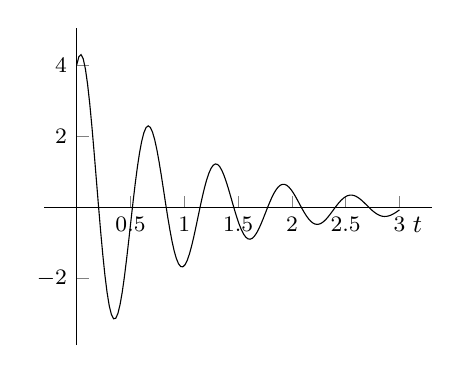
\begin{tikzpicture}
\begin{axis}[small,axis lines*=middle,xlabel={$t$},xlabel style={at={(current axis.right of origin)},anchor=north east}]
\addplot[domain=0:3,samples=150]{e^(-x)*(4*cos(180/pi*10*x)+2*sin(180/pi*10*x))};
\end{axis}
\end{tikzpicture}
\caption{قصری ارتعاش (مثال \حوالہ{مثال_لاپلاس_بدل_قصری_ارتعاش})}
\label{شکل_لاپلاس_قصری_ارتعاش}
\end{figure}
\انتہا{مثال}
%=======================

\جزوحصہء{لاپلاس بدل کی وجودیت اور یکتائی}
اگر تمام  \عددی{t \ge 0} کے لئے، کسی مستقل \عددی{k} اور \عددی{M} پر تفاعل \عددی{f} \موٹا{بڑھنے کی پابندی}
\begin{align}\label{مساوات_لاپلاس_بڑھنے_کی_حد}
\abs{f(t)} \le M e^{kt}
\end{align}
پر پورا اترتا ہو، تب اس کا لاپلاس بدل موجود ہو گا۔ہم کہتے ہیں کہ نہایت تیزی سے نہ بڑھنے والے  تفاعل \عددی{f(t)} کا لاپلاس بدل موجود ہو گا۔

\عددی{f(t)} کا استمراری  ہونا ضروری نہیں ہے البتہ اس کا \اصطلاح{ٹکڑوں میں استمراری}\فرہنگ{استمراری!ٹکڑوں میں}\حاشیہب{piecewise continuous}\فرہنگ{continuous!piecewise} ہونا لازم ہے۔  اگر محدود وقفہ \عددی{a \le t \le b} جس پر \عددی{f(t)} معین ہو، کو کئی ایسے ٹکڑوں میں تقسیم کرنا ممکن ہو کہ ہر ٹکڑے پر \عددی{f(t)} استمراری ہو اور \عددی{t} کا اندرون ٹکڑے سے ٹکڑے کے (دونوں) سروں تک پہنچنے پر  \عددی{f(t)} کی قیمت کا \اصطلاح{حد}\حاشیہب{limit} محدود حاصل ہو تب \عددی{f(t)} \اصطلاح{ٹکڑوں میں استمراری} کہلائے گا۔ ایسی صورت میں، جیسا شکل \حوالہ{شکل_لاپلاس_ٹکڑوں_استمراری} میں دکھایا گیا ہے، محدود \اصطلاح{چھلانگ}\فرہنگ{چھلانگ}\حاشیہب{jumps}\فرہنگ{jumps} پائے جائیں گے جو غیر استمراری صورت کی واحد وجہ ہو گی۔ عموماً عملی مسائل اسی نوعیت کے ہوتے ہیں۔درج ذیل مسئلہ بھی اسی نوعیت کا ہے۔ 
\begin{figure}
\centering
\begin{tikzpicture}
%axis
\draw(0,-1)--(0,2);
\draw(0,0)--++(6,0)node[right]{$t$};
\draw(1,0)--++(0,-0.1)node[below]{$a$};
\draw(5,0)--++(0,-0.1)node[below]{$b$};
%piecewise continuous
\draw(1,0.5) to [out=30,in=-150]++(1,1)node[circ]{};
\draw(2,2) to [out=-20,in=120]++(1,-2.5)node[circ]{};
\draw(3,0.3) to [out=0,in=-145]++(1,0.5)coordinate(kA);
\draw(4,1.4)coordinate(kB)--++(0.4,0)--++(0.6,-0.5);
\draw($(kA)!0.5!(kB)$) node[circ]{};
\end{tikzpicture}
\caption{ٹکڑوں میں استمراری تفاعل \عددی{f(t)}۔ غیر استمراری مقام پر تفاعل کی قیمت کو نقطوں سے ظاہر کیا گیا ہے۔}
\label{شکل_لاپلاس_ٹکڑوں_استمراری}
\end{figure}
%=============

\ابتدا{مسئلہ}\شناخت{مسئلہ_لاپلاس_وجودیت}\quad مسئلہ وجودیت لاپلاس بدل\\
اگر نصف محور \عددی{t \ge 0} کے ہر محدود وقفے پر تفاعل \عددی{f(t)} معین اور ٹکڑوں میں استمراری ہو اور مساوات \حوالہ{مساوات_لاپلاس_بڑھنے_کی_حد} پر، 
تمام \عددی{t \ge 0} اور کسی مستقل \عددی{M} اور \عددی{k} کے لئے،  پورا اترتا ہو تب لاپلاس بدل \عددی{\Laplace (f)} تمام \عددی{s >k} کے لئے موجود ہو گا ۔ 
\انتہا{مسئلہ}
%=========================

\ابتدا{ثبوت}
چونکہ \عددی{f(t)} ٹکڑوں میں استمراری ہے لہٰذا \عددی{t} محور کے کسی بھی محدود وقفے پر \عددی{e^{-st}f(t)} قابل تکمل ہے۔ مساوات \حوالہ{مساوات_لاپلاس_بڑھنے_کی_حد} کو دیکھ کر، \عددی{s>k} تصور کرتے ہوئے (جو درج ذیل آخری تکمل میں درکار ہے)، لاپلاس بدل کی وجودیت کا ثبوت حاصل کرتے ہیں۔
\begin{align*}
\abs{\Laplace(f)} = \abs{\int_{0}^{\infty} e^{-st}f(t)\dif t}\le \int_{0}^{\infty} \abs{f(t)}e^{-st}\dif t\le \int_{0}^{\infty} Me^{kt}e^{-st}\dif t=\frac{M}{s-k}
\end{align*}
\انتہا{ثبوت}
%=========================

کسی بھی تفاعل کا مساوات \حوالہ{مساوات_لاپلاس_بڑھنے_کی_حد} میں دیے گئے شرط پر پورا اترنے کو با آسانی دیکھا جا سکتا ہے، مثلاً \عددی{\cosh t < e^t} یا \عددی{t^n<n!e^t} (چونکہ \عددی{\tfrac{t^n}{n!}} مکلارن تسلسل کا ایک رکن ہے)۔ ایسا تفاعل جو مساوات \حوالہ{مساوات_لاپلاس_بڑھنے_کی_حد} پر پورا نہ اترتا ہو کی مثال \عددی{e^{t^2}} ہے۔آپ سوال \حوالہ{سوال_لاپلاس_کافی} میں دیکھیں گے کہ مسئلہ \حوالہ{مسئلہ_لاپلاس_وجودیت} میں دیے گئے شرائط لاپلاس بدل کی وجودیت کے لئے کافی ہیں نا کہ لازمی ہیں۔

\جزوحصہء{یکتائی}
اگر کسی تفاعل کا لاپلاس بدل موجود ہو تو یہ بدل یکتا ہو گا۔اسی طرح اگر (حقیقی مثبت محور پر معین) دو تفاعل کے لاپلاس بدل یکساں ہوں تب یہ تفاعل، کسی بھی مثبت لمبائی کے وقفے پر،  آپس میں مختلف نہیں ہو سکتے ہیں، البتہ تنہا نقطوں پر ان کی قیمت غیر یکساں ہو سکتی ہے۔یوں ہم کہہ سکتے ہیں کہ الٹ لاپلاس بدل یکتا ہے۔ بالخصوص دو ایسے استمراری تفاعل جن کا لاپلاس بدل یکساں ہو، آپس میں مکمل طور پر یکساں ہوں گے۔ 
%========================

\حصہء{سوالات}
%=============
سوال \حوالہ{سوال_لاپلاس_بدل_الف} تا سوال \حوالہ{سوال_لاپلاس_بدل_ب} میں لاپلاس بدل حاصل کریں۔ \عددی{a} اور  \عددی{b} کو مستقل تصور کریں۔

\ابتدا{سوال}\شناخت{سوال_لاپلاس_بدل_الف}\quad
$2t-3$\\
جواب:\عددی{\tfrac{2}{s^2}-\tfrac{3}{s}}
\انتہا{سوال}
%=======================
\ابتدا{سوال}\quad
$(at+b)^2$\\
جواب:\عددی{a(\tfrac{b}{s^2}+\tfrac{2a}{s^3})+b(\tfrac{b}{s}+\tfrac{a}{s^2})}
\انتہا{سوال}
%=====================
\ابتدا{سوال}\quad
$\sin 2\pi t$\\
جواب:\عددی{\tfrac{2\pi}{s^2+4\pi^2}}
\انتہا{سوال}
%====================
\ابتدا{سوال}\quad
$\sin^2 2\pi t$\\
جواب:\عددی{\tfrac{8\pi^2}{s(s^2+16\pi^2)}}
\انتہا{سوال}
%====================
\ابتدا{سوال}\quad
$e^{-3t}\sin 4t$\\
جواب:\عددی{\tfrac{4}{(s+3)^2+16}}
\انتہا{سوال}
%======================
\ابتدا{سوال}\quad
$e^{2t}\cos 3t$\\
جواب:\عددی{\tfrac{s-2}{(s-2)^2+9}}
\انتہا{سوال}
%======================
\ابتدا{سوال}\quad
$\cos (2t-\frac{\pi}{3})$\\
جواب:\عددی{\tfrac{\tfrac{s}{2}+\sqrt{3}}{s^2+4}}
\انتہا{سوال}
%=========================
\ابتدا{سوال}\شناخت{سوال_لاپلاس_بدل_ب} \quad
$2\sin (5t+\pi)$\\
جواب:\عددی{\tfrac{-10}{s^2+25}}
\انتہا{سوال}
%======================
\begin{figure}
\centering
\begin{subfigure}{0.33\textwidth}
\centering
\begin{tikzpicture}
%axis
\draw[gray](0,0)--(0,1.5);
\draw[gray](0,0)--(3,0);
%function
\draw[thick](0,0)--(2,1);
\draw[dashed](2,1)--(2,0);
\draw[thick](2,0)node[below]{$2$}--(3,0);
\draw(0,1)--++(-0.1,0)node[left]{$1$};
\draw(1,-0.5)node{(الف)};
\end{tikzpicture}%
\end{subfigure}%
\begin{subfigure}{0.33\textwidth}
\centering
\begin{tikzpicture}
%axis
\draw[gray](0,0)--(0,1.5);
\draw[gray](0,0)--(3,0);
%function
\draw[thick](0,1)--(2,1);
\draw[dashed](2,1)--(2,0)node[below]{$3$};
\draw[thick](2,0)--(3,0);
\draw(0,1)--++(-0.1,0)node[left]{$2$};
\draw(1,-0.5)node{(ب)};
\end{tikzpicture}%
\end{subfigure}%
\begin{subfigure}{0.33\textwidth}
\centering
\begin{tikzpicture}
%axis
\draw[gray](0,0)--(0,1.5);
\draw[gray](0,0)--(3,0);
%function
\draw[thick](0,1)--(2,0);
\draw[thick](2,0)node[below]{$5$}--(3,0);
\draw(0,1)--++(-0.1,0)node[left]{$2$};
\draw(1,-0.5)node{(پ)};
\end{tikzpicture}%
\end{subfigure}
%
\begin{subfigure}{0.33\textwidth}
\centering
\begin{tikzpicture}
%axis
\draw[gray](0,-1.2)--(0,1.2);
\draw[gray](0,0)--(3,0);
%function
\draw[thick](0,1)--(2,-1);
\draw[dashed](2,-1)--(2,0);
\draw[thick](2,0)node[above]{$2$}--(3,0);
\draw(0,1)--++(-0.1,0)node[left]{$5$};
\draw(0,-1)--++(-0.1,0)node[left]{$-5$};
\draw(0.75,-0.75)node{(ت)};
\end{tikzpicture}%
\end{subfigure}%
\begin{subfigure}{0.33\textwidth}
\centering
\begin{tikzpicture}
%axis
\draw[gray](0,0)--(0,1.5);
\draw[gray](0,0)--(3,0);
%function
\draw[thick](0,0)--(1,1)--(2.5,0)node[below]{$7$}--(3,0);
\draw(0,1)--++(-0.1,0)node[left]{$2$};
\draw(1,0)--++(0,-0.1)node[below]{$3$};
\draw(1,-0.75)node{(ٹ)};
\end{tikzpicture}%
\end{subfigure}%
\begin{subfigure}{0.33\textwidth}
\centering
\begin{tikzpicture}
%axis
\draw[gray](0,0)--(0,1.5);
\draw[gray](0,0)--(3,0);
%function
\draw[thick](0,0)--(1,1);
\draw[dashed](1,1)--(1,1.5);
\draw[thick](1,1.5)--(2,1.5);
\draw[dashed](2,1.5)--(2,0);
\draw[thick](2,0)node[below]{$4$}--(3,0);
\draw(0,1)--++(-0.1,0)node[left]{$2$};
\draw(0,1.5)--++(-0.1,0)node[left]{$3$};
\draw(1,0)--++(0,-0.1)node[below]{$2$};
\draw(1.5,-0.75)node{(ث)};
\end{tikzpicture}%
\end{subfigure}
\caption{سوال \حوالہ{سوال_لاپلاس_بدل_پ} تا سوال \حوالہ{سوال_لاپلاس_بدل_پ} کے اشکال۔}
\label{شکل_سوال_لاپلاس_بدل_پ}
\end{figure}
%================
\ابتدا{سوال}\شناخت{سوال_لاپلاس_بدل_پ} 
شکل \حوالہ{شکل_سوال_لاپلاس_بدل_پ}-الف میں ٹکڑوں میں استمراری تفاعل دکھایا گیا ہے۔تمام ٹکڑوں کی ریاضی مساوات حاصل کریں۔ تکمل \حوالہ{مساوات_لاپلاس_بدل_الف}  کو ٹکڑوں میں تقسیم کرتے ہوئے لاپلاس بدل حاصل کریں۔

جواب:\عددی{\tfrac{1-e^{-2s}(2s+1)}{2s^2}}
\انتہا{سوال}
%=========================
\ابتدا{سوال}
شکل \حوالہ{شکل_سوال_لاپلاس_بدل_پ}-ب میں دیے گئے تفاعل کا لاپلاس بدل حاصل کریں۔

جواب:\عددی{\tfrac{2}{s}(1-e^{-3s})}
\انتہا{سوال}
%===========================
\ابتدا{سوال}
شکل \حوالہ{شکل_سوال_لاپلاس_بدل_پ}-پ میں دیے گئے تفاعل کا لاپلاس بدل حاصل کریں۔

جواب:\عددی{\tfrac{2e^{-5s}+10s-2}{5s^2}}
\انتہا{سوال}
%===========================
\ابتدا{سوال}
شکل \حوالہ{شکل_سوال_لاپلاس_بدل_پ}-ت میں دیے گئے تفاعل کا لاپلاس بدل حاصل کریں۔

جواب:\عددی{\tfrac{5(s+1)e^{-2s}+5(s-1)}{s^2}}
\انتہا{سوال}
%===========================
\ابتدا{سوال}
شکل \حوالہ{شکل_سوال_لاپلاس_بدل_پ}-ٹ میں دیے گئے تفاعل کا لاپلاس بدل حاصل کریں۔

جواب:\عددی{\tfrac{4-7e^{-3s}+3e^{-7s}}{6s^2}}
\انتہا{سوال}
%===========================
\ابتدا{سوال}
شکل \حوالہ{شکل_سوال_لاپلاس_بدل_پ}-ث میں دیے گئے تفاعل کا لاپلاس بدل حاصل کریں۔

جواب:\عددی{\tfrac{1+(s-1)e^{-2s}-3se^{-4s}}{s^2}}
\انتہا{سوال}
%===========================
\ابتدا{سوال}\شناخت{سوال_لاپلاس_کافی}\quad وجودیت\\
تفاعل \عددی{\tfrac{1}{\sqrt{t}}} کا لاپلاس بدل حاصل کریں۔ایسا کرتے ہوئے \عددی{\Gamma(\tfrac{1}{2})=\sqrt{\pi}} (مساوات \حوالہ{مساوات_بیسل_گیما_نیم}) کا استعمال کریں۔ اس سے آپ اخذ کر سکتے ہیں کہ مسئلہ \حوالہ{مسئلہ_لاپلاس_وجودیت} میں دیے شرائط کافی ہیں نا کہ لازمی۔

جواب:\عددی{\tfrac{\sqrt{\pi}}{s}}
\انتہا{سوال}
%==============================
\ابتدا{سوال}
\عددی{e^{at}} کا لاپلاس بدل \عددی{\cosh at} اور \عددی{\sinh at} کے لاپلاس بدل سے حاصل کریں۔

جواب:\عددی{e^{at}=\sinh at+\cosh at} لکھ کر جواب \عددی{\tfrac{1}{s-a}} ملتا ہے۔
\انتہا{سوال}
%============================
\ابتدا{سوال}\quad پیمائشی فیتہ میں ردوبدل\\
ثابت کریں کہ اگر \عددی{\Laplace[f(t)]=F(s)}  ہو تب \عددی{\Laplace[f(ct)]=\tfrac{F(\tfrac{s}{c})}{c}} ہو گا جہاں \عددی{c} مستقل ہے۔اس کلیے کو استعمال کرتے ہوئے \عددی{\Laplace(\cos t)} سے \عددی{\Laplace(\cos \omega t)} حاصل کریں۔

جواب:مساوات \حوالہ{مساوات_لاپلاس_بدل_الف} استعمال کرتے ہوئے کلیہ ثابت ہو گا۔
\انتہا{سوال}
%=============================
\ابتدا{سوال}\quad الٹ لاپلاس بدل کی خطیت\\
\عددی{\Laplace} کی خطیت کو استعمال کرتے ہوئے ثابت کریں کہ \عددی{\Laplace^{-1}} خطی ہے۔
\انتہا{سوال}
%==============================
سوال \حوالہ{سوال_لاپلاس_الٹ_الف} تا سوال \حوالہ{سوال_لاپلاس_الٹ_ب} میں الٹ لاپلاس بدل حاصل کریں۔

%==============
\ابتدا{سوال}\شناخت{سوال_لاپلاس_الٹ_الف}\quad
$\frac{0.5s+1.3}{s^2+1.69}$\\
جواب:\عددی{\sin (1.3t)+0.5\cos(1.3t)}
\انتہا{سوال}
%========================
\ابتدا{سوال}\quad
$\frac{4s+1}{s^2-16}$\\
جواب:\عددی{\tfrac{1}{8}(17e^{4t}+15e^{-4t})}
\انتہا{سوال}
%========================
\ابتدا{سوال}\quad
$\frac{s}{m^2s^2+n^2}$\\
جواب:\عددی{\tfrac{\cos \tfrac{nt}{m}}{m^2}}
\انتہا{سوال}
%=========================
\ابتدا{سوال}\quad
$\frac{1}{(s+3)(s-2)}$\\
جواب:\عددی{\tfrac{1}{5}(e^{2t}-e^{-3t})}
\انتہا{سوال}
%========================
\ابتدا{سوال}\quad
$\frac{2}{s^3}+\frac{3}{s^5}$\\
جواب:\عددی{t^2+\tfrac{t^4}{8}}
\انتہا{سوال}
%======================
\ابتدا{سوال}\quad
$\frac{3s+8}{s^2-9}$\\
جواب:\عددی{\tfrac{1}{6}(17e^{3t}+e^{-3t})}
\انتہا{سوال}
%========================
\ابتدا{سوال}\quad
$\frac{s-1}{s^2-s-6}$\\
جواب:\عددی{\tfrac{1}{5}(2e^{3t}+3e^{-2t})}
\انتہا{سوال}
%=======================
\ابتدا{سوال}\شناخت{سوال_لاپلاس_الٹ_ب}\quad
$\frac{1}{(s-a)(s+b)}$\\
جواب:\عددی{\tfrac{1}{a+b}(e^{at}-e^{-bt})}
\انتہا{سوال}
%=====================
سوال \حوالہ{سوال_لاپلاس_منتقلی_الف} تا سوال \حوالہ{سوال_لاپلاس_منتقلی_ت} منتقلی \عددی{s} پر مبنی ہیں۔ سوال \حوالہ{سوال_لاپلاس_منتقلی_الف} تا سوال \حوالہ{سوال_لاپلاس_منتقلی_ب} میں لاپلاس بدل جبکہ سوال \حوالہ{سوال_لاپلاس_منتقلی_پ} تا سوال \حوالہ{سوال_لاپلاس_منتقلی_ت} میں الٹ لاپلاس بدل حاصل کریں۔

%=========
\ابتدا{سوال}\شناخت{سوال_لاپلاس_منتقلی_الف}\quad
$te^{2t}$\\
جواب:\عددی{\tfrac{1}{(s-2)^2}}
\انتہا{سوال}
%=======================
\ابتدا{سوال}\quad
$e^{-3t}\sin 5t$\\
جواب:\عددی{\tfrac{5}{(s+3)^2+5^2}}
\انتہا{سوال}
%==========================
\ابتدا{سوال}\quad
$0.25e^{-1.5t}\cos (3\pi t)$\\
جواب:\عددی{\tfrac{0.25(s+1.5)}{(s+1.5)^2+(3\pi)^2}}
\انتہا{سوال}
%=============================
\ابتدا{سوال}\شناخت{سوال_لاپلاس_منتقلی_ب}\quad
$\sinh t \sin \omega t$\\
جواب:\عددی{\tfrac{1}{2}[\tfrac{\omega}{(s-1)^2+\omega^2}-\tfrac{\omega}{(s+1)^2+\omega^2}]}
\انتہا{سوال}
%============================
\ابتدا{سوال}\شناخت{سوال_لاپلاس_منتقلی_پ}\quad
$\frac{m}{(s+n)^2}$\\
جواب:\عددی{mte^{-nt}}
\انتہا{سوال}
%=============================
\ابتدا{سوال}\quad
$\frac{3}{(s+5)^4}$\\
جواب:\عددی{\tfrac{t^3e^{-5t}}{2}}
\انتہا{سوال}
%===================
\ابتدا{سوال}\quad
$\tfrac{3}{(s+\sqrt{5})^3}$\\
جواب:\عددی{\tfrac{3t^2e^{-\sqrt{5}t}}{2}}
\انتہا{سوال}
%========================
\ابتدا{سوال}\quad
$\tfrac{4}{s^2+2s+5}$\\
جواب:\عددی{2e^{-t}\sin 2t}
\انتہا{سوال}
%======================
\ابتدا{سوال}\quad
$\frac{\pi}{s^2+8\pi s+17\pi^2}$\\
جواب:\عددی{e^{-4\pi t}\sin \pi t}
\انتہا{سوال}
%========================
\ابتدا{سوال}\quad
$\frac{3s+22}{s^2+8s+41}$\\
جواب:\عددی{e^{-4t}(2\sin 5t+3\cos 5t)}
\انتہا{سوال}
%=============================
\ابتدا{سوال}\quad
$\frac{s+a+b}{(s+a)^2+b^2}$\\
جواب:\عددی{e^{-at}(\cos bt+\sin bt)}
\انتہا{سوال}
%=======================
\ابتدا{سوال}\شناخت{سوال_لاپلاس_منتقلی_ت}\quad
$\frac{a}{s+c}+\frac{b}{(s+c)^2}$\\
جواب:\عددی{(a+bt)e^{-ct}}
\انتہا{سوال}
%=======================

\حصہ{تفرقات اور تکملات کے لاپلاس بدل۔ سادہ تفرقی مساوات}
لاپلاس بدل کو استعمال کرتے ہوئے سادہ تفرقی مساوات اور ابتدائی قیمت مسائل حل کیے جاتے ہیں۔لاپلاس بدل کے استعمال سے  احصائی اعمال کی جگہ الجبرائی اعمال استعمال کیے جاتے ہیں۔یوں \عددی{f(t)} کا تفرق، \عددی{F(s)} کو \عددی{s} سے ضرب دینے کے (تقریباً) مترادف ہو گا جبکہ \عددی{f(t)} کا تکمل،  \عددی{F(s)} کو \عددی{s} سے تقسیم کرنے کے مترادف ہو گا۔ 
%====================
\ابتدا{مسئلہ}\شناخت{مسئلہ_لاپلاس_ایک_درجی}\quad \عددی{f(t)} کی تفرق کا لاپلاس بدل\\
اگر \عددی{f(t)} تمام \عددی{t \ge 0} پر استمراری ہو، مساوت \حوالہ{مساوات_لاپلاس_بڑھنے_کی_حد} پر پورا اترتا ہو اور \عددی{f'(t)} نصف محور \عددی{t \ge 0} کے ہر محدود وقفے پر \اصطلاح{ٹکڑوں میں استمراری} ہو تب، \عددی{s>k} کی صورت میں، \عددی{f'(t)} کا لاپلاس بدل موجود ہو گا جو درج ذیل سے حاصل کیا جا سکتا ہے۔
\begin{align} \label{مساوات_لاپلاس_درجہ_اول_تفرق}
\Laplace(f')&=s\Laplace(f)-f(0)\quad \quad (s>k)
\end{align}
\انتہا{مسئلہ}
%=======================

\ابتدا{ثبوت}
ہم یہ  فرض کرتے ہوئے  کہ \عددی{f'} \موٹا{بھی} استمراری ہے مساوات \حوالہ{مساوات_لاپلاس_درجہ_اول_تفرق} ثابت کرتے ہیں۔یوں لاپلاس بدل کی تعریف (مساوات \حوالہ{مساوات_لاپلاس_بدل_الف}) اور تکمل بالحصص سے درج ذیل لکھا جا سکتا ہے۔
\begin{align*}
\Laplace(f')=\int_{0}^{\infty} e^{-st} f'(t)\dif t=\left. e^{-st} f(t) \right|_{0}^{\infty}+s\int_{0}^{\infty} e^{-st}f(t)\dif t=f(0)+sF(s)
\end{align*}
چونکہ \عددی{f(t)} مساوات \حوالہ{مساوات_لاپلاس_بڑھنے_کی_حد} پر پورا اترتی ہے لہٰذا \عددی{s>k} کی صورت میں  \عددی{t=\infty} پر \عددی{e^{-st}f(t)}صفر دیگا جبکہ \عددی{t=0} پر یہ \عددی{f(0)} دیگا۔آخری تکمل \عددی{\Laplace (f)=F(s)} کے برابر ہے  جس کا حل، \عددی{s>k} کی  صورت میں، مسئلہ \حوالہ{مسئلہ_لاپلاس_وجودیت} کے تحت موجود ہے۔یوں \عددی{\Laplace(f')} کا حل موجود ہے۔

اگر \عددی{f'} ٹکڑوں میں استمراری ہو تب درج بالا ثبوت میں تکمل کو ایسے ٹکڑوں میں تقسیم کیا جاتا ہے کہ ہر ٹکڑے (وقفے) پر \عددی{f'} استمراری ہو۔ سوال \حوالہ{سوال_لاپلاس_مسئلہ_تفرق} میں اس پر غور کیا گیا ہے۔
\انتہا{ثبوت}
%===========================

\عددی{f''} پر مساوات \حوالہ{مساوات_لاپلاس_درجہ_اول_تفرق}  لاگو کر کے حاصل جواب میں مساوات \حوالہ{مساوات_لاپلاس_درجہ_اول_تفرق} پر کرتے ہوئے درج ذیل ملتا ہے۔
\begin{align}\label{مساوات_لاپلاس_درجہ_دوم_تفرق}
\Laplace(f'')=s\Laplace(f')-f'(0)=s[s\Laplace(f)-f(0)]-f'(0)=s^2\Laplace(f)-sf(0)-f'(0)
\end{align}
اسی ترکیب کو \عددی{f'''} پر لاگو کرتے ہوئے
\begin{align}\label{مساوات_لاپلاس_درجہ_تین_تفرق}
\Laplace(f''')=s^3\Laplace(f)-s^2f(0)-sf'(0)-f''(0)
\end{align}
ملتا ہے۔اس ترکیب کو بار بار استعمال کرتے ہوئے درج ذیل مسئلہ اخذ کیا جا سکتا ہے۔
%=======================

\ابتدا{مسئلہ}\شناخت{مسئلہ_لاپلاس_بلند_درجی}\quad بلند درجی تفرق \عددی{f^n}\\
اگر \عددی{f(t)} اور اس کے تفرقات \عددی{f'(t)}، \عددی{f''(t)}، \نقطے، \عددی{f^{(n-1)}(t)}  تمام \عددی{t \ge 0} پر استمراری ہوں، مساوت \حوالہ{مساوات_لاپلاس_بڑھنے_کی_حد} پر پورا اترتے ہوں اور \عددی{f^{(n)}(t)} نصف محور \عددی{t \ge 0} کے ہر محدود وقفے پر \اصطلاح{ٹکڑوں میں استمراری} ہو تب، \عددی{s>k} کی صورت میں، \عددی{f^{(n)}(t)} کا لاپلاس بدل موجود ہو گا جو درج ذیل سے حاصل کیا جا سکتا ہے۔
\begin{align}
\Laplace(f^{(n)})=s^n\Laplace(f)-s^{n-1}f(0)-s^{n-2}f'(0)-\cdots -f^{(n-1)}(0)
\end{align}
\انتہا{مسئلہ}
%=============================

\ابتدا{مثال}
تفاعل \عددی{f(t)=t^2} کا لاپلاس بدل حاصل کریں۔

حل:\عددی{f'=2t} اور \عددی{f''=2} ہیں۔یوں \عددی{f(0)=0}، \عددی{f'(0)=0} اور \عددی{f''(0)=2} ملتے ہیں۔اب \عددی{\Laplace(2)=\tfrac{2}{s}} ہے لہٰذا  مساوات \حوالہ{مساوات_لاپلاس_درجہ_دوم_تفرق} استعمال کرتے ہوئے درج ذیل لکھا جا سکتا ہے جو جدول \حوالہ{جدول_لاپلاس_بدل_الف} کے عین مطابق ہے۔
\begin{align*}
\Laplace(f'')=\Laplace(2)=\frac{2}{s}=s^2\Laplace(f), \quad \implies \quad \Laplace(t^2)=\frac{2}{s^3}
\end{align*}
عموماً کسی بھی تفاعل کا لاپلاس بدل کئی مختلف طریقوں سے حاصل کرنا ممکن ہوتا ہے۔
\انتہا{مثال}
%=============================
\ابتدا{مثال}\شناخت{مثال_لاپلاس_مربع_سائن}
تفاعل \عددی{f(t)=\sin^2 t} کا لاپلاس بدل حاصل کریں۔

حل:\عددی{f(0)=0} ہے جبکہ \عددی{f'=2\sin t \cos t=\sin 2t} لکھا جا سکتا ہے۔یوں مساوات \حوالہ{مساوات_لاپلاس_درجہ_اول_تفرق} استعمال کرتے ہوئے درج ذیل لکھا جا سکتا ہے۔ 
\begin{align*}
\Laplace(\sin 2t)=\frac{2}{s^2+4}=s\Laplace(f) \quad \implies \quad \Laplace(f)=\frac{2}{s(s^2+4)}
\end{align*}
\انتہا{مثال}
%==============================
\ابتدا{مثال}
تفاعل \عددی{f(t)=t\sin \omega t} کا لاپلاس بدل حاصل کریں۔

حل:\عددی{f(0)=0} ہے جبکہ
\begin{align*}
f'(t)&=\sin \omega t-\omega t\cos \omega t, \quad f'(0)=0,\\
f''(t)&=2\omega \cos \omega t-\omega^2 t \sin \omega t=2\omega \cos \omega t-\omega^2 f(t)
\end{align*}
ہیں۔یوں مساوات \حوالہ{مساوات_لاپلاس_درجہ_دوم_تفرق} استعمال کرتے ہوئے
\begin{align*}
\Laplace(f'')=2\omega \Laplace(\cos \omega t)-\omega^2\Laplace(f)=s^2\Laplace(f)
\end{align*}
لکھا جا سکتا ہے جس میں \عددی{\cos \omega t} کا لاپلاس بدل پر کرتے 
\begin{align*}
(s^2+\omega^2)\Laplace(f)=2\omega \Laplace(\cos \omega t)=\frac{2\omega s}{s^2+\omega^2}
\end{align*}
ہوئے درج ذیل حاصل کرتے ہیں۔
\begin{align*}
\Laplace(t\sin \omega t)=\frac{2\omega s}{(s^2+\omega^2)^2}
\end{align*}
\انتہا{مثال}
%==============================
\ابتدا{مثال}\شناخت{مثال_لاپلاس_کوسائن_ضرب_وقت}
تفاعل \عددی{f(t)=t\cos \omega t} کا لاپلاس بدل حاصل کریں۔

حل:ہم درج ذیل لکھ سکتے ہیں۔
\begin{align*}
f(t)&=t\cos \omega t, \quad f(0)=0\\
f'(t)&=\cos \omega t-\omega t\sin \omega t, \quad f'(0)=1\\
f''(t)&=-2\omega \sin \omega t-\omega^2 f(t)
\end{align*}
یوں مساوات \حوالہ{مساوات_لاپلاس_درجہ_دوم_تفرق} استعمال کرتے ہوئے درج ذیل لکھا جا سکتا ہے۔
\begin{align*}
\Laplace(f'')&=s^2\Laplace(f)-sf(0)-sf'(0)\\
&=s^2F(s)-1
\end{align*}
ساتھ ہی ساتھ \عددی{f''} کی مساوات کا لاپلاس بدل درج ذیل لکھا جا سکتا ہے۔
\begin{align*}
\Laplace(f'')&=\Laplace[-2\omega \sin \omega t-\omega^2 f(t)]\\
&=-\frac{2\omega^2}{s^2+\omega^2}-\omega^2F(s)
\end{align*}
ان دونوں جوابات کو برابر پر کرتے ہوئے درج ذیل ملتا ہے۔
\begin{align}\label{مساوات-لاپلاس_کوسائن_ضرب_وقت}
F(s)=\Laplace[t\cos \omega t]=\frac{s^2-\omega^2}{(s^2+\omega^2)^2}
\end{align}
\انتہا{مثال}
%===============================
\ابتدا{مثال}\شناخت{مثال_لاپلاس_ٹکڑوں_میں_استمراری}
استمراری \عددی{f(t)} کی صورت میں  \عددی{f'(t)} کا لاپلاس بدل مسئلہ \حوالہ{مسئلہ_لاپلاس_ایک_درجی} دیتی ہے۔آئیں \اصطلاح{ٹکڑوں میں استمراری} \عددی{f(t)} کی صورت میں \عددی{f'(t)} کا لاپلاس بدل حاصل کریں۔شکل \حوالہ{شکل_مثال_لاپلاس_ٹکڑوں_میں_استمراری} کے تفاعل میں \عددی{t=a(>0)} پر تفاعل غیر استمراری ہے جبکہ بقایا تمام شرائط وہی ہیں جو مسئلہ \حوالہ{مسئلہ_لاپلاس_ایک_درجی} میں تھے۔اس تفاعل کا لاپلاس بدل حاصل کریں۔
\begin{figure}
\centering
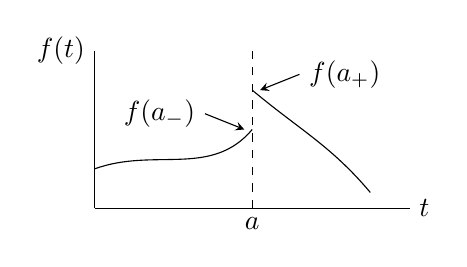
\begin{tikzpicture}
%axis
\draw(0,0)--++(0,2)node[left]{$f(t)$};
\draw(0,0)--(4,0)node[right]{$t$};
\draw(0,0.5) to [out=20,in=-130]++(2,0.5)coordinate(kL);
\draw(2,1.5)coordinate(kR) to [out=-40,in=130]++(1.5,-1.3);
\draw[stealth-] (kL)++(-0.1,0)--++(-0.5,0.2)node[left]{$f(a_-)$};
\draw[stealth-] (kR)++(0.1,0)--++(0.5,0.2)node[right]{$f(a_+)$};
\draw[dashed](2,0)node[below]{$a$}--++(0,2);
\end{tikzpicture}
\caption{ٹکڑوں میں استمراری تفاعل \عددی{f(t)}(مثال \حوالہ{مثال_لاپلاس_ٹکڑوں_میں_استمراری})}
\label{شکل_مثال_لاپلاس_ٹکڑوں_میں_استمراری}
\end{figure}

شکل \حوالہ{شکل_مثال_لاپلاس_ٹکڑوں_میں_استمراری} میں دکھایا گیا تفاعل \عددی{t=a} غیر استمراری ہے۔ ہم کہتے ہیں کہ \عددی{t=a} پر تفاعل \اصطلاح{چھلانگ}\فرہنگ{چھلانگ}\حاشیہب{jump}\فرہنگ{jump} لگاتا ہے یا کہ تفاعل میں \عددی{t=0} پر \اصطلاح{چھلانگ} پائی جاتی ہے۔نقطہ چھلانگ تک بائیں جانب سے پہنچتے ہوئے تفاعل کے قیمت کی \اصطلاح{حد}\فرہنگ{حد}\حاشیہب{limit}\فرہنگ{limit} کو \عددی{f(a_{-})} لکھا جاتا ہے جبکہ نقطہ چھلانگ تک دائیں جانب سے پہنچتے ہوئے تفاعل کے قیمت کی حد کو \عددی{f(a_+)} لکھا جاتا ہے۔یوں \عددی{t=a} پر تفاعل کی چھلانگ \عددی{f(a_+)-f(a_-)} ہو گی۔

لاپلاس بدل کی تعریف (مساوات \حوالہ{مساوات_لاپلاس_بدل_الف}) سے درج ذیل لکھا جا سکتا ہے جہاں تکمل کو ایسے ٹکڑوں (وقفوں) میں تقسیم کیا گیا ہے کہ ہر وقفے پر \عددی{f(t)} استمراری ہے۔
\begin{align*}
\Laplace(f')=\int_{a_+}^{\infty} e^{-st}f' \dif t+\int_{0}^{a_-}e^{-st}f' \dif t
\end{align*}  
پہلے تکمل کا ابتدائی حد \عددی{a_+} ہے جو \عددی{t=a} کے دائیں طرف کو ظاہر کرتی ہے جہاں تفاعل کی قیمت \عددی{f(a_+)}  ہے۔اسی طرح دوسری تکمل کا اختتامی حد \عددی{a_-} ہے جس پر تفاعل کی قیمت \عددی{f(a_-)} ہے۔انہیں شکل میں دکھایا گیا ہے۔  تکمل بالحصص سے
\begin{align*}
\Laplace(f')&=\left. e^{-st} f(t)\right|_{a_+}^{\infty}+s\int_{a_+}^{\infty}e^{-st}f(t)\dif t+\left. e^{-st}f(t) \right|_{0}^{a_-}+s\int_{0}^{a_-}e^{-st} f(t)\dif t\\
&=-e^{-sa}f(a_+)+s\int_{a_+}^{\infty}e^{-st}f(t)\dif t+e^{-sa}f(a_-)-f(0)+s\int_{0}^{a_-}e^{-st} f(t)\dif t\\
&=s\int_{0}^{\infty}e^{-st}f(t)\dif t -f(0)-e^{-sa}[f(a_+)-f(a_-)]\\
&=sF(s) -f(0)-e^{-sa}[f(a_+)-f(a_-)]
\end{align*}
حاصل ہوتا ہے جہاں \عددی{e^{-st}} استمراری ہونے کی بدولت  \عددی{e^{-sa_+}=s^{-sa_-}=s^{-sa}} ہے۔
\انتہا{مثال}
%==================================
\ابتدا{مثال}\quad تفرقی مساوات\\
درج ذیل ابتدائی قیمت مسئلہ حل  کریں۔
\begin{align*}
y''+3y'+2y=0, \quad y(0)=2, \quad y'(0)=-1
\end{align*} 
حل: \موٹا{پہلا قدم} ضمنی مساوات کا حصول ہے۔تا معلوم تفاعل \عددی{y(t)} کا لاپلاس بدل \عددی{َY(s)=\Laplace(y)} لکھ کر مساوات \حوالہ{مساوات_لاپلاس_درجہ_اول_تفرق} اور مساوات \حوالہ{مساوات_لاپلاس_درجہ_دوم_تفرق} میں دیے گئے ابتدائی معلومات پر کرتے ہوئے درج ذیل لکھا جا سکتا ہے۔
\begin{align*}
\Laplace(y')&=sY-y(0)=sY-2\\
\Laplace(y'')&=s^2Y-sy(0)-y'(0)=s^2Y-2s+1
\end{align*}
انہیں دیے گئے تفرقی مساوات میں پر کرتے ہوئے درج ذیل ملتا ہے۔\عددی{Y} کی مساوات کو \اصطلاح{ضمنی مساوات}\فرہنگ{ضمنی مساوات}\فرہنگ{مساوات!ضمنی}\حاشیہب{subsidiary equation}\فرہنگ{subsidiary equation} کہتے ہیں۔
\begin{align*}
s^2Y+3sY+2Y=2s+5
\end{align*}
\موٹا{دوسرا قدم} ضمنی مساوات کا الجبرائی حل ہے۔موجودہ ضمنی مساوات کو
\begin{align*}
(s+1)(s+2)Y=2s+5
\end{align*}
لکھ کر جزوی کسری پھیلاو کی مدد سے  درج ذیل لکھ سکتے ہیں۔
\begin{align*}
Y=\frac{2s+5}{(s+1)(s+2)}=\frac{3}{s+1}-\frac{1}{s+2}
\end{align*}
\موٹا{تیسرا قدم} الٹ لاپلاس بدل حاصل کرنا ہے۔جدول \حوالہ{جدول_لاپلاس_بدل_الف} سے 
\begin{align*}
\Laplace^{-1}\left[\frac{3}{s+1}\right]=3e^{-t}, \quad \Laplace^{-1}\left[\frac{1}{s+2}\right]=e^{-2t}
\end{align*}
لکھا جا سکتا ہے۔یوں خطیت (مسئلہ \حوالہ{مسئلہ_لاپلاس_خطیت}) استعمال کرتے ہوئے  دیے گئے ابتدائی قیمت مسئلے کا حل لکھتے ہیں۔
\begin{align*}
y(t)=\Laplace^{-1}[Y]=3e^{-t}-e^{-2t}
\end{align*}
\انتہا{مثال}
%===================================
درج بالا مثال میں آپ نے دیکھا کہ لاپلاس بدل سے تفرقی مساوات کے حل میں شروع سے  ابتدائی قیمتیں مسئلے کا حصہ بنتی ہیں۔

\جزوحصہء{تفاعل کے تکمل کا لاپلاس بدل}
ہم نے دیکھا کہ تفاعل کے تفرق کا لاپلاس بدل، اصل تفاعل کے لاپلاس بدل کو \عددی{s} سے ضرب دینے کے (تقریباً) مترادف ہے۔چونکہ تکمل اور تفرق آپس میں الٹ اعمال ہیں لہٰذا ہم توقع کرتے ہیں کہ تفاعل کے تکمل کا لاپلاس بدل، اصل تفاعل کے لاپلاس بدل تقسیم \عددی{s} ہو گا۔ 

%=======================
\ابتدا{مسئلہ}\شناخت{مسئلہ_لاپلاس_تکمل_کا_بدل}\quad \عددی{f(t)} کی تکمل کا لاپلاس بدل\\
اگر \عددی{f(t)} ٹکڑوں میں استمراری ہو اور مساوات \حوالہ{مساوات_لاپلاس_بڑھنے_کی_حد} پر پورا اترتا ہو تب درج ذیل ہو گا۔
\begin{align}\label{مساوات_لاپلاس_تکمل_کا_بدل}
\Laplace\left[\int_{0}^{t} f(\tau) \dif \tau \right]=\frac{1}{s}\Laplace[f(t)]\quad \quad (s>0, \, s>k)
\end{align} 
\انتہا{مسئلہ}
%=======================

\ابتدا{ثبوت}
فرض کریں کہ \عددی{f(t)} ٹکڑوں میں استمراری ہے اور مساوات \حوالہ{مساوات_لاپلاس_بڑھنے_کی_حد} پر پورا اترتی ہے۔اب گر منفی \عددی{k} کے لئے  مساوات \حوالہ{مساوات_لاپلاس_بڑھنے_کی_حد} کی شرط پوری ہوتی ہو تب مثبت \عددی{k} کے لئے بھی یہ شرط پوری ہو گی۔ہم فرض کرتے ہیں کہ \عددی{k} مثبت ہے لہٰذا تکمل
\begin{align}\label{مساوات_لاپلاس_تفاعل_تکمل}
g(t)=\int_{0}^{t}f(\tau)\dif \tau
\end{align}
استمراری ہو گا اور مساوات \حوالہ{مساوات_لاپلاس_بڑھنے_کی_حد} کے استعمال سے
\begin{align*}
\abs{g(t)}\le \int_{0}^{t} \abs{f(\tau)} \dif \tau \le M\int_{0}^{t} e^{k\tau} \dif \tau=\frac{M}{k}(e^{kt}-1)\quad \quad (k>0)
\end{align*}
لکھا جا سکتا ہے۔مزید ماسوائے ان نقطوں پر جہاں \عددی{f(t)} غیر استمراری ہو، \عددی{g'(t)=f(t)} ہو گا۔اس طرح \عددی{g'(t)} ہر محدود وقفے پر \اصطلاح{ٹکڑوں میں استمراری} ہو گا لہٰذا مسئلہ \حوالہ{مسئلہ_لاپلاس_ایک_درجی} کے تحت
\begin{align*}
\Laplace[f(t)]=\Laplace[g'(t)]=s\Laplace[g(t)]-g(0) \quad \quad (s>k)
\end{align*}
ہو گا۔اب مساوات \حوالہ{مساوات_لاپلاس_تفاعل_تکمل} سے \عددی{g(0)=0} ملتا ہے لہٰذا \عددی{\Laplace(f)=s\Laplace(g)} ہو گا جو مساوات \حوالہ{مساوات_لاپلاس_تکمل_کا_بدل} ہی ہے۔
\انتہا{ثبوت}
%========================

مساوات \حوالہ{مساوات_لاپلاس_تکمل_کا_بدل} میں \عددی{\Laplace[f(t)]=F(s)} لکھ کر اور اطراف بدل کر، الٹ لاپلاس بدل لینے سے
\begin{align}\label{مساوات_لاپلاس_تکمل_کا_بدل_جڑواں}
\Laplace^{-1}\left[\frac{F(s)}{s}\right]=\int_{0}^{t} f(\tau)\dif \tau
\end{align}
حاصل ہوتا ہے جو مساوات \حوالہ{مساوات_لاپلاس_تکمل_کا_بدل} کی جڑواں مساوات ہے۔

%==============
\ابتدا{مثال}\شناخت{مثال_لاپلاس_دو_درجی_تکمل}
\عددی{\frac{1}{s^2(s^2+\omega^2)}} کا الٹ لاپلاس بدل لیتے ہوئے تفاعل \عددی{f(t)} حاصل کریں۔

حل:جدول \حوالہ{جدول_لاپلاس_بدل_الف} 
\begin{align*}
\Laplace^{-1}\left(\frac{1}{s^2+\omega^2}\right)=\frac{1}{\omega}\sin \omega t
\end{align*}
دیتی ہے۔یوں مسئلہ \حوالہ{مسئلہ_لاپلاس_تکمل_کا_بدل} استعمال کرتے ہوئے
\begin{align*}
\Laplace^{-1}\left[\frac{1}{s}\left(\frac{1}{s^2+\omega^2}\right)\right]=\frac{1}{\omega} \int_{0}^{t}\sin \omega \tau \dif \tau=\frac{1}{\omega^2} (1-\cos \omega t)
\end{align*}
حاصل ہو گا۔مسئلہ \حوالہ{مسئلہ_لاپلاس_تکمل_کا_بدل} ایک مرتبہ دوبارہ استعمال کرتے ہوئے درج ذیل حاصل ہو گا۔
\begin{align*}
\Laplace^{-1}\left[\frac{1}{s^2} \left(\frac{1}{s^2+\omega^2}\right)\right]=\frac{1}{\omega^2} \int_{0}^{t}(1-\cos \omega \tau) \dif \tau=\frac{1}{\omega^2}\left(t-\frac{\sin \omega t}{\omega}\right)
\end{align*}
\انتہا{مثال}
%==========================

\حصہء{سوالات}

%==================================
\ابتدا{سوال}
\عددی{\sin^2 t} کا لاپلاس بدل مثال \حوالہ{مثال_لاپلاس_مربع_سائن} میں حاصل کیا گیا۔یہاں \عددی{\sin^2 t=\tfrac{1}{2}(1-\cos 2t)} لکھ کر لاپلاس بدل دوبارہ حاصل کریں۔

جواب:\عددی{\tfrac{1}{2}[\tfrac{1}{s}-\tfrac{s}{s^2+4}]=\tfrac{2}{s(s^2+4)}}
\انتہا{سوال}
%===========================
\ابتدا{سوال}
\عددی{\cos^2 t} کا لاپلاس بدل مثال \حوالہ{مثال_لاپلاس_مربع_سائن} کی طرز پر حاصل کریں۔

جواب:\عددی{\tfrac{s^2+2}{s(s^2+4)}}
\انتہا{سوال}
%========================
\ابتدا{سوال}
\عددی{\cos^2 t=1-\sin^2 t} لکھ کر \عددی{\cos^2 t} کا لاپلاس بدل حاصل کریں۔

جواب:\عددی{\tfrac{s^2+2}{s(s^2+4)}}
\انتہا{سوال}
%=======================
\ابتدا{سوال}
ہم نے مثال \حوالہ{مثال_لاپلاس_دو_درجی_تکمل} میں الٹ لاپلاس بدل حاصل کیا۔اسی کو درج ذیل لکھ کر دوبارہ الٹ لاپلاس بدل حاصل کریں۔
\begin{align*}
\frac{1}{s^2(s^2+\omega^2)}=\frac{1}{\omega^2}\left(\frac{1}{s^2}-\frac{1}{s^2+\omega^2}\right)
\end{align*}
\انتہا{سوال}
%=========================
\ابتدا{سوال}
مسئلہ \حوالہ{مسئلہ_لاپلاس_ایک_درجی} استعمال کرتے ہوئے \عددی{\sin \omega t} کے لاپلاس بدل سے \عددی{\cos \omega t} کا لاپلاس بدل حاصل کریں۔ 
\انتہا{سوال}
%============================
\ابتدا{سوال}
تفاعل \عددی{f(t)=\sin \omega t} کا لاپلاس بدل بذریعہ مساوات \حوالہ{مساوات_لاپلاس_درجہ_دوم_تفرق} حاصل کریں۔

جواب:\عددی{f(0)=0} ہے جبکہ \عددی{f'=\omega \cos \omega t} اور \عددی{f''=-\omega^2\sin\omega t=-\omega^2 f} ہیں۔یوں \عددی{f'(0)=\omega} ملتا ہے۔ مساوات \حوالہ{مساوات_لاپلاس_درجہ_دوم_تفرق} سے \عددی{\Laplace (f'')=-\omega^2\Laplace (f)=s^2\Laplace (f)-s(0)-\omega} لکھا جائے گا جس سے جدول \حوالہ{جدول_لاپلاس_بدل_الف} میں دیا گیا جواب  \عددی{\Laplace(f)=\tfrac{\omega}{s^2+\omega^2}} ملتا ہے۔
\انتہا{سوال}
%==================================
\ابتدا{سوال}
تفاعل \عددی{f(t)=\cos \omega t} کا لاپلاس بدل بذریعہ مساوات \حوالہ{مساوات_لاپلاس_درجہ_دوم_تفرق} حاصل کریں۔جدول سے جواب دیکھیں۔
\انتہا{سوال}
%==============================
\ابتدا{سوال}
مسئلہ \حوالہ{مسئلہ_لاپلاس_بلند_درجی} استعمال کرتے ہوئے \عددی{f(t)=t^n} کا لاپلاس بدل حاصل کریں  جہاں \عددی{t} عدد صحیح ہے۔

جواب:چونکہ \عددی{f(0)=0}، \عددی{f'(0)=0}، \نقطے،  \عددی{f^{(n-1)}(0)=0} ہیں جبکہ \عددی{f^{n}=n!} ہے لہٰذا مسئلہ \حوالہ{مسئلہ_لاپلاس_بلند_درجی} سے  \عددی{\Laplace(f^{n})=s^nF(s)} لکھا جائے گا جبکہ \عددی{\Laplace(f^{(n)})=\Laplace(n!)=\tfrac{n!}{s}} ہے۔یوں \عددی{\Laplace(t^n)=\tfrac{n!}{s^{n+1}}} حاصل ہوتا ہے۔
\انتہا{سوال}
%============================
\ابتدا{سوال}\شناخت{سوال_لاپلاس_سائن_ضرب_وقت}
ہم نے مثال \حوالہ{مثال_لاپلاس_کوسائن_ضرب_وقت} میں \عددی{t\cos \omega t} کا لاپلاس بدل حاصل کیا۔اسی طرز پر \عددی{t\sin \omega t} کا لاپلاس بدل حاصل کریں۔

جواب:\عددی{\tfrac{2\omega s}{(s^2+\omega^2)^2}}
\انتہا{سوال}
%============================
\ابتدا{سوال}
\عددی{t\sinh a t} کا لاپلاس بدل حاصل کریں۔

جواب:\عددی{\tfrac{2as}{(s^2-a^2)^2}}
\انتہا{سوال}
%============================
\ابتدا{سوال}
\عددی{t\cosh a t} کا لاپلاس بدل حاصل کریں۔

جواب:\عددی{\tfrac{s^2+a^2}{(s^2-a^2)^2}}
\انتہا{سوال}
%============================
\ابتدا{سوال}\شناخت{سوال_لاپلاس_الٹ_بدل_سوال_الف}
مثال \حوالہ{مثال_لاپلاس_کوسائن_ضرب_وقت} اور سوال \حوالہ{سوال_لاپلاس_سائن_ضرب_وقت} میں بالترتیب \عددی{t\cos \omega t} اور \عددی{t\sin \omega t} کا لاپلاس بدل حاصل کیا گیا۔انہیں استعمال کرتے ہوئے درج ذیل حاصل کریں۔
\begin{align}
\Laplace^{-1}\left[\frac{1}{(s^2+\omega^2)^2}\right]&=\frac{1}{2\omega^3}(\sin \omega t-\omega t \cos \omega t)
\end{align}
جواب:\عددی{t\sin \omega t} کے بدل سے \عددی{\Laplace^{-1}\tfrac{2\omega s}{(s^2+\omega^2)^2}=t\sin \omega t} لکھا جا سکتا ہے جسے استعمال کرتے ہوئے مسئلہ \حوالہ{مسئلہ_لاپلاس_تکمل_کا_بدل} سے \عددی{\Laplace^{-1}\tfrac{2\omega}{(s^2+\omega^2)^2}=\int_{0}^{t}\tau\sin \omega \tau\dif \tau} ملتا ہے۔دائیں ہاتھ تکمل بالحصص سے \عددی{\tfrac{\sin \omega t}{\omega^3}-\tfrac{t\cos \omega t}{\omega^2}} ملتا ہے۔ان نتائج کو اکٹھے کرتے ہوئے درکار جواب حاصل ہوتا ہے۔
\انتہا{سوال}
%============================
\ابتدا{سوال}
درج ذیل ثابت کریں۔سوال \حوالہ{سوال_لاپلاس_الٹ_بدل_سوال_الف} کی طرز پر حل کریں۔
\begin{align}
\Laplace^{-1}\left[\frac{s^2}{(s^2+\omega^2)^2}\right]&=\frac{1}{2\omega}(\sin \omega t+\omega t\cos \omega t)
\end{align}
\انتہا{سوال}
%===============================
\ابتدا{سوال}\شناخت{سوال_لاپلاس_مسئلہ_تفرق}
\عددی{f'(t)} میں محدود چھلانگ نقطہ \عددی{t_1}، \عددی{t_2}، \نقطے، \عددی{t_n} پر پائے جاتے ہیں جبکہ \عددی{f(t)} استمراری ہے۔  \عددی{t_1<t_2<\cdots <t_n}  لیتے ہوئے  مسئلہ \حوالہ{مسئلہ_لاپلاس_ایک_درجی} ثابت کریں۔  

جواب:
\begin{multline*}
\Laplace(f')=\int_{0}^{t_{1-}}e^{-st} f' \dif t+\int_{t_{1+}}^{t_{2-}}e^{-st} f' \dif t+\int_{t_{2+}}^{t_{3-}}e^{-st} f' \dif t+\cdots+\int_{t_{n+}}^{\infty}e^{-st} f' \dif t
\end{multline*}
لکھ کر تکمل بالحصص حاصل کرتے ہیں۔
\begin{multline}\label{مساوات_سوال_مسئلہ_ایک_درجی}
\Laplace(f')=\left. e^{-st}f(t)\right|_{0}^{t_{1-}}+s\int_{0}^{t_{1-}}e^{-st}f(t)\dif t+\left. e^{-st}f(t)\right|_{t_{1+}}^{t_{2-}}+s\int_{t_{1+}}^{t_{2-}}e^{-st}f(t)\dif t\\
+\left. e^{-st}f(t)\right|_{t_{2+}}^{t_{3-}}+s\int_{t_{2+}}^{t_{3-}}e^{-st}f(t)\dif t+\cdots+\left. e^{-st}f(t)\right|_{t_{n+}}^{\infty}+s\int_{t_{n+}}^{\infty}e^{-st}f(t)\dif t
\end{multline}
اب \عددی{f(t)} استمراری ہے لہٰذا مساوات \حوالہ{مساوات_سوال_مسئلہ_ایک_درجی} میں متعدد تکملات کو یکجا کیا جا سکتا ہے
\begin{align*}
s\int_{0}^{t_{1-}}e^{-st}f(t)\dif t+s\int_{t_{1+}}^{t_{2-}}e^{-st}f(t)\dif t+\cdots +s\int_{t_{n+}}^{\infty}e^{-st}f(t)\dif t=s\int_{0}^{\infty}e^{-st}f(t)\dif t
\end{align*}
جبکہ بقایا اجزاء سے درج ذیل ملتا ہے۔
\begin{multline*}
e^{(-st_{1-})}f(t_{1-})-f(0)+e^{(-st_{2-})}f(t_{2-})-e^{(-st_{1+})}f(t_{1+})+e^{(-st_{3-})}f(t_{3-})\\
-e^{(-st_{2+})}f(t_{2+})+\cdots+e^{(-\infty)}f(\infty)-e^{(-st_{n+})}f(t_{n+})
\end{multline*}
چونکہ \عددی{f(t)} استمراری ہے لہٰذا  \عددی{e^{(-st_{m-})}f(t_{m-})=e^{(-st_{m+})}f(t_{m+})=e^{(-st_m)}f(t_m)} ہو گا۔یوں \عددی{e^{(-st_{1-})}f(t_{1-})} اور \عددی{-e^{(-st_{1+})}f(t_{1+})} آپس میں کٹ جائیں گے۔اسی طرح بقایا اجزاء بھی آپس میں کٹ جاتے ہیں۔پہلے دو اجزاء میں سے \عددی{f(0)} بچتا ہے جبکہ  \عددی{f(t)} محدود تفاعل ہونے کی بنا \عددی{e^{-\infty}f(\infty)=0} ہو گا۔اس طرح مسئلہ \حوالہ{مسئلہ_لاپلاس_ایک_درجی} کا ثبوت مکمل ہوتا ہے۔
\انتہا{سوال}
%==============================
سوال \حوالہ{سوال_لاپلاس_تکمل_بدل_الف} تا سوال \حوالہ{سوال_لاپلاس_تکمل_بدل_ب} کو مسئلہ \حوالہ{مسئلہ_لاپلاس_تکمل_کا_بدل} کی مدد سے حل کریں۔

%===========================
\ابتدا{سوال}\شناخت{سوال_لاپلاس_تکمل_بدل_الف}\quad
$\tfrac{1}{s^2+s}$\\
جواب:\عددی{1-e^{-t}}
\انتہا{سوال}
%==============================
\ابتدا{سوال}\quad
$\tfrac{6}{s^2+4s}$\\
جواب:\عددی{\tfrac{3}{2}(1-e^{-4t})}
\انتہا{سوال}
%========================
\ابتدا{سوال}\quad
$\tfrac{3}{s^2-9s}$\\
جواب:\عددی{\tfrac{1}{3}(e^{9t}-1)}
\انتہا{سوال}
%=====================
\ابتدا{سوال}\quad
$\tfrac{9}{s^3+9s}$\\
جواب:\عددی{1-\cos 3t}
\انتہا{سوال}
%=====================
\ابتدا{سوال}\quad
$\tfrac{4}{s^2(s+2)}$\\
جواب:\عددی{e^{-2t}+2t-1}
\انتہا{سوال}
%========================
\ابتدا{سوال}\quad
$\tfrac{4}{s^3(s+2)}$\\
جواب:\عددی{-\tfrac{e^{-2t}}{2}+t^2-t+\tfrac{1}{2}}
\انتہا{سوال}
%========================
\ابتدا{سوال}\quad
$\tfrac{12}{s(s^2+4)}$\\
جواب:\عددی{3-3\cos 2t}
\انتہا{سوال}
%====================
\ابتدا{سوال}\quad
$\tfrac{12}{s^2(s^2+4)}$\\
جواب:\عددی{3t-\tfrac{3}{2}\sin 2t}
\انتہا{سوال}
%====================
\ابتدا{سوال}\quad
$\tfrac{32}{s(s^2-16)}$\\
جواب:\عددی{2\cosh 4t-2}
\انتہا{سوال}
%=======================
\ابتدا{سوال}\quad
$\tfrac{32}{s^2(s^2-16)}$\\
جواب:\عددی{\tfrac{1}{2}\sinh 4t-2t}
\انتہا{سوال}
%======================
\ابتدا{سوال}\شناخت{سوال_لاپلاس_تکمل_بدل_ب}\quad
$\tfrac{6}{s^4(s^2+1)}$\\
جواب:\عددی{6\sin t+t^3-6t}
\انتہا{سوال}
%=======================
لاپلاس بدل استعمال کرتے ہوئے ابتدائی قیمت سوالات \حوالہ{سوال_لاپلاس_ابتدائی_الف} تا \حوالہ{سوال_لاپلاس_ابتدائی_ب} حل کریں۔

%==============
\ابتدا{سوال}\شناخت{سوال_لاپلاس_ابتدائی_الف}\quad
$y''+\pi^2y=0,\quad y(0)=1, \, y'(0)=0$\\
جواب:\عددی{y=\cos \pi t}
\انتہا{سوال}
%=======================
\ابتدا{سوال}\quad
$y''+\omega^2 y=0,\quad y(0)=A,\, y'(0)=B$\\
جواب:\عددی{y=A\cos \omega t+\tfrac{B}{\omega}\sin \omega t}
\انتہا{سوال}
%=========================
\ابتدا{سوال}\quad
$y''-5y'+6y=0,\quad y(0)=1, \, y'(0)=-1$\\
جواب:\عددی{y=4e^{2t}-3e^{3t}}
\انتہا{سوال}
%=======================

\ابتدا{سوال}\quad
$y''-y'-2y=0,\quad y(0)=2, \, y'(0)=1$\\
جواب:\عددی{y=e^{2t}+e^{-t}}
\انتہا{سوال}
%=======================
\ابتدا{سوال}\quad
$y''-2y'+y=0,\quad y(0)=2,\, y'(0)=1$\\
جواب:\عددی{y=(2-t)e^t}
\انتہا{سوال}
%=======================
\ابتدا{سوال}\quad
$y''-ky'=0,\quad y(0)=2, \, y'(0)=k, \, k>0$\\
جواب:\عددی{y=1+e^{kt}}
\انتہا{سوال}
%=========================
\ابتدا{سوال}\شناخت{سوال_لاپلاس_ابتدائی_ب}\quad
$y''+ky'-2k^2y=0,\quad y(0)=2,\, y'(0)=2k$\\
جواب:\عددی{y=2e^{kt}}
\انتہا{سوال}
%===========================
\ابتدا{سوال}\quad جبری، بلا تقصیر ارتعاش\\
ثابت کریں کہ درج ذیل
\begin{align*}
y''+\omega^2y=r(t)
\end{align*}
کے ضمنی مساوات کا حل درج ذیل ہے جہاں \عددی{r(t)} کا لاپلاس بدل \عددی{R(s)} ہے۔  \عددی{\omega} مستقل ہے اور \عددی{r(t)} جبری تفاعل ہے۔
\begin{align*}
Y(s)=\frac{sy(0)+y'(0)}{s^2+\omega^2}+\frac{R(s)}{s^2+\omega^2}
\end{align*}
دھیان رہے کہ جواب کا پہلا جزو صرف اور صرف ابتدائی معلومات پر منحصر ہے جبکہ جواب کے دوسرے جزو پر ابتدائی معلومات کا کوئی اثر نہیں پایا جاتا ہے۔ 
\انتہا{سوال}
%=====================

\حصہ{\عددی{s} محور پر منتقلی، \عددی{t} محور پر منتقلی، اکائی سیڑھی تفاعل}
اب تک ہم لاپلاس بدل کے کئی خواص جان چکے ہیں۔ اس حصے میں دو مزید خصوصیات پیش کیے جائیں گے جنہیں \عددی{s} محور پر منتقلی (مسئلہ \حوالہ{مسئلہ_لاپلاس_تعددی_محور_منتقلی}) اور \عددی{t} محور پر منتقلی (مسئلہ \حوالہ{مسئلہ_لاپلاس_وقتی_محور_منتقلی}) کہتے ہیں۔

%===========================
\ابتدا{مسئلہ}\شناخت{مسئلہ_لاپلاس_تعددی_محور_منتقلی}\quad \عددی{s} محور پر منتقلی؛ منتقلی کا پہلا مسئلہ\\
اگر \عددی{f(t)} کا لاپلاس بدل \عددی{F(s)} ہو جہاں \عددی{s>k} ہے، تب \عددی{e^{at}f(t)} کا لاپلاس بدل \عددی{F(s-a)} ہو گا جہاں \عددی{s-a>k} ہے۔یوں اگر
\begin{align*}
\Laplace[f(t)]=F(s)
\end{align*}
ہو تب 
\begin{align*}
\Laplace[e^{at}f(t)]=F(s-a)
\end{align*}
ہو گا۔یوں اصل تفاعل کو \عددی{e^{at}} سے ضرب دینا، لاپلاس بدل میں \عددی{s} کی جگہ \عددی{s-a} پر کرنے کے مترادف ہے یعنی لاپلاس بدل \عددی{s} محور پر اپنی جگہ سے سرک کر نئی جگہ منتقل ہو جاتا ہے (شکل \حوالہ{شکل_لاپلاس_تعددی_منتقلی} دیکھیں)۔ 
\begin{figure}
\centering
\begin{tikzpicture}
%axis
\draw(0,0)--(0,2);
\draw(0,0)--(4,0)node[right]{$s$};
%transform
\draw(0.5,1.3)coordinate(kL) to [out=-60, in=170]++(2,-1);
\draw(1.5,1.3)coordinate(kR) to [out=-60, in=170]++(2,-1);
%
\draw[dashed](kL)++(0,0.1)--++(0,0.3);
\draw[dashed](kR)++(0,0.1)--++(0,0.3);
\draw[stealth-stealth](kL)++(0,0.1+0.15)--++(1,0)node[pos=0.5,fill=white]{$a$};
\end{tikzpicture}
\caption{منتقلی کا پہلا مسئلہ، \عددی{s} محور پر منتقلی}
\label{شکل_لاپلاس_تعددی_منتقلی}
\end{figure}
\انتہا{مسئلہ}
%==========================
\ابتدا{ثبوت}
لاپلاس بدل کی تعریف
\begin{align*}
F(s)=\int_{0}^{\infty}e^{-st} f(t)\dif t
\end{align*}
استعمال کرتے ہوئے \عددی{s} کی جگہ \عددی{s-a} پر کرتے ہیں۔
\انتہا{ثبوت}
\begin{align*}
F(s-a)=\int_{0}^{\infty}e^{-(s-a)t} f(t)\dif t=\int_{0}^{\infty}e^{-st} [e^{at}f(t)]\dif t=\Laplace[e^{at}f(t)]
\end{align*}
%==========================

\ابتدا{مثال}
منتقلی کا پہلا مسئلہ استعمال کرتے ہوئے جدول \حوالہ{جدول_لاپلاس_بدل_الف} میں درج  تفاعل \عددی{t^n}، \عددی{\sin \omega t} اور \عددی{\cos \omega t} کو \عددی{e^{at}} سے ضرب دے کر لاپلاس بدل لکھتے ہیں۔
\begin{align*}
\Laplace[e^{at}t^n]&=\frac{n!}{(s-a)^{n+1}}\\
\Laplace[e^{at}\sin \omega t]&=\frac{\omega}{(s-a)^2+\omega^2}\\
\Laplace[e^{at}\cos \omega t]&=\frac{s-a}{(s-a)^2+\omega^2}
\end{align*} 
\انتہا{مثال}
%================================
\ابتدا{مثال}\quad قصری آزاد ارتعاش\\
چھت سے لٹکی  لچکدار اسپرنگ کے نچلے سرے سے کمیت \عددی{m=3} لٹکائی گئی ہے۔اسپرنگ کا ینگ مقیاس لچک \عددی{k=6} ہے۔کمیت کے ساکن مقام سے فاصلہ \عددی{y(t)}  ہے۔کمیت کو ابتدائی طور پر \عددی{y(0)=4} پر رکھ کر اس کو ابتدائی رفتار \عددی{y'(0)=-3} دی جاتی ہے۔فرض کریں کہ کمیت کی رفتار کے راست متناسب قصری قوت عمل کرتی ہے جہاں قصری مستقل \عددی{c=12} کے برابر ہے۔کمیت کی حرکت دریافت کریں۔

حل:کمیت کی حرکت کو درج ذیل ابتدائی قیمت مسئلہ بیان کرتا ہے
\begin{align*}
y''+2y'+4y=0,\quad \quad y(0)=4, \, y'(0)=-3
\end{align*}
جس کا ضمنی مساوات 
\begin{align*}
s^2Y-4s+3+2(sY-4)+4Y=0
\end{align*}
ہے۔ضمنی مساوات کا حل لکھتے ہیں۔
\begin{align*}
Y=\frac{4s+5}{s^2+2s+4}=\frac{4(s+1)}{(s+1)^2+3}+\frac{1}{(s+1)^2+3}
\end{align*}
اب ہم جانتے ہیں کہ
\begin{align*}
\Laplace^{-1}\left(\frac{s}{s^2+3}\right)=\cos \sqrt{3}t, \quad \quad \Laplace^{-1}\left(\frac{\sqrt{3}}{s^2+3}\right)=\sin \sqrt{3}t
\end{align*}
ہیں لہٰذا مسئلہ \حوالہ{مسئلہ_لاپلاس_تعددی_محور_منتقلی} کی مدد سے حل لکھتے ہیں۔
\begin{align*}
y(t)=\Laplace^{-1}(Y)=e^{-t}(4\cos \sqrt{3}t+\frac{1}{\sqrt{3}}\sin \sqrt{3}t)
\end{align*}
\انتہا{مثال}
%===================================

\جزوحصہء{\عددی{t} محور پر منتقلی، اکائی سیڑھی تفاعل}
منتقلی کے پہلے مسئلے میں ہم نے دیکھا کہ تفاعل \عددی{f(t)} کو \عددی{e^{at}} سے ضرب دینا، لاپلاس بدل میں \عددی{s} کی جگہ \عددی{s-a} لکھنے کے مترادف ہے۔اب ہم منتقلی کا دوسرا مسئلہ (مسئلہ \حوالہ{مسئلہ_لاپلاس_وقتی_محور_منتقلی}) پیش کرتے ہیں جس کے تحت تفاعل \عددی{f(t)} میں \عددی{t} کی جگہ \عددی{t-a} پر کرنا، لاپلاس بدل \عددی{F(s)} کو (تقریباً) \عددی{e^{-as}} سے ضرب دینے کے مترادف ہے۔

%=======================
\ابتدا{مسئلہ}\شناخت{مسئلہ_لاپلاس_وقتی_محور_منتقلی}\quad \عددی{t} محور پر منتقلی؛ منتقلی کا دوسرا مسئلہ\\
اگر تفاعل \عددی{f(t)} کا لاپلاس بدل \عددی{F(s)} ہو تب \عددی{e^{-as}F(s)}، جہاں \عددی{a>0} ہے، درج ذیل تفاعل کا لاپلاس بدل ہو گا۔
\begin{align*}
\tilde{f}(t)=
\begin{cases}
0& t<a\\
f(t-a) &  t>a
\end{cases}
\end{align*}
\موٹا{ہیوی سائیڈ سیڑھی تفاعل}\فرہنگ{ہیوی سائیڈ سیڑھی تفاعل}\حاشیہب{Heaviside step function}\فرہنگ{Heaviside step function}، جسے شکل \حوالہ{شکل_لاپلاس_اکائی_سیڑھی_تفاعل} میں دکھایا گیا ہے، کی تعریف\حاشیہد{الیور ہیوی سائیڈ [1850-1925] خود لکھ پڑھ کر برقی مہندس، ریاضی دان اور ماہر طبیعیات بنے۔یہ انگلستانی تھے۔} درج ذیل ہے۔ہیوی سائیڈ سیڑھی تفاعل کو \اصطلاح{اکائی سیڑھی تفاعل}\فرہنگ{اکائی!سیڑھی تفاعل}\فرہنگ{سیڑھی!اکائی}\حاشیہب{unit step function}\فرہنگ{step!function} بھی  کہتے ہیں۔
\begin{align}
u(t-a)=
\begin{cases}
0 & t<a\\
1& t>a
\end{cases}
\end{align}
\عددی{t<a} پر اکائی سیڑھی تفاعل کی قیمت صفر ہے جبکہ \عددی{t>a} پر اس کی قیمت اکائی ہے۔عین \عددی{t=a} پر اکائی سیڑھی تفاعل \اصطلاح{غیر معین}\فرہنگ{غیر معین}\حاشیہب{undefined}\فرہنگ{undefined} ہے اور یہاں اس میں اکائی کی چھلانگ پائی جاتی ہے۔

اکائی سیڑھی تفاعل کو زیر استعمال لاتے ہوئے ہم \عددی{\tilde{f}(t)} کو \عددی{f(t-a)u(t-a)} لکھ سکتے ہیں جس کی مثال شکل \حوالہ{شکل_لاپلاس_سیڑھی_ضرب_تفاعل} میں دکھائی گئی ہے۔اس طرح مسئلہ \حوالہ{مسئلہ_لاپلاس_وقتی_محور_منتقلی}  کہتا ہے کہ
\begin{align}\label{مساوات_لاپلاس_منتقلی_وقت_صورت_الف}
e^{-as}F(s)=\Laplace[f(t-a)u(t-a)]
\end{align}
جسے الٹ لاپلاس بدل لیتے ہوئے درج ذیل لکھا جا سکتا ہے۔
\begin{align}\label{مساوات_لاپلاس_منتقلی_وقت_صورت_ب}
\Laplace^{-1}[e^{-as}F(s)]=f(t-a)u(t-a)
\end{align}
%
\begin{figure}
\centering
\begin{tikzpicture}
%axis
\draw(-1,0)--(4,0)node[right]{$t$};
\draw(0,0)--++(0,1.5)node[left]{$u(t-a)$};
%step
\draw[thick](-1,0)--(1,0)node[below]{$a$};
\draw[dashed](1,0)--(1,1);
\draw[thick](1,1)--(4,1);
\draw(0,1)--++(-0.1,0)node[left]{$1$};
\end{tikzpicture}
\caption{اکائی سیڑھی تفاعل \عددی{u(t-a)}}
\label{شکل_لاپلاس_اکائی_سیڑھی_تفاعل}
\end{figure}
%
\begin{figure}
\centering
\begin{subfigure}{0.5\textwidth}
\centering
\begin{tikzpicture}
\begin{axis}[small,axis lines*=middle,xlabel={$t$},ylabel={${f(t)=\sin t}$},xlabel style={at={(current axis.right of origin)},anchor=north east},ylabel style={rotate=-90},ylabel style={at={(current axis.above origin)},anchor=south west},xtick=\empty,ytick=\empty]
\addplot[domain=0:360]{sin(x)};
\addplot[]plot coordinates{(0,0)}node[ocirc]{};
\end{axis}
\end{tikzpicture}
\end{subfigure}%
\begin{subfigure}{0.5\textwidth}
\centering
\begin{tikzpicture}
\begin{axis}[small,axis lines*=middle,xlabel={$t$},ylabel={$f(t-a)$},xlabel style={at={(current axis.right of origin)},anchor=north east},ylabel style={rotate=-90},ylabel style={at={(current axis.above origin)},anchor=south west},xtick=\empty,ytick=\empty]
\addplot[domain=0:360]{sin(x-80)};
\addplot[dashed] plot coordinates {(80,0) (80,0.5)};
\addplot[]plot coordinates{(80,0)}node[ocirc]{}node[below right]{$a$};
\addplot[stealth-stealth] plot coordinates {(0,0.3) (80,0.3)}node[pos=0.5,fill=white]{$a$};
\end{axis}
\end{tikzpicture}
\end{subfigure}
\begin{subfigure}{0.5\textwidth}
\centering
\begin{tikzpicture}
\begin{axis}[small,axis lines*=middle,xlabel={$t$},ylabel={$u(t-a)$},xlabel style={at={(current axis.right of origin)},anchor=north east},ylabel style={rotate=-90},ylabel style={at={(current axis.above origin)},anchor=south west},xtick={80},xticklabels={$a$},ytick=\empty]
\addplot[] plot coordinates {(0,0) (80,0) (80,1) (360,1) };
\end{axis}
\end{tikzpicture}
\end{subfigure}%
\begin{subfigure}{0.5\textwidth}
\centering
\begin{tikzpicture}
\begin{axis}[small,axis lines*=middle,xlabel={$t$},ylabel={${f(t-a)u(t-a)}$},xlabel style={at={(current axis.right of origin)},anchor=north east},ylabel style={rotate=-90},ylabel style={at={(current axis.above origin)},anchor=south west},xtick={80},xticklabels={$a$},ytick=\empty]
\addplot[] plot coordinates {(0,0) (80,0) };
\addplot[domain=80:360]{sin(x-80)};
\end{axis}
\end{tikzpicture}
\end{subfigure}
\caption{\عددی{f(t-a)u(t-a)} جہاں \عددی{f(t)=\sin t} ہے۔}
\label{شکل_لاپلاس_سیڑھی_ضرب_تفاعل}
\end{figure}
\انتہا{مسئلہ}
%==================
\ابتدا{ثبوت}\quad مسئلہ \حوالہ{مسئلہ_لاپلاس_وقتی_محور_منتقلی} کا ثبوت\\
لاپلاس بدل کی تعریف سے 
\begin{align*}
e^{-as}F(s)=e^{-as}\int_{0}^{\infty}e^{-s\tau}f(\tau)\dif \tau=\int_{0}^{\infty}e^{-s(\tau+a)}f(\tau)\dif \tau
\end{align*}
لکھا جا سکتا ہے جس میں \عددی{\tau+a=t} پر کرتے ہوئے
\begin{align*}
e^{-as}F(s)=\int_{a}^{\infty}e^{-st}f(t-a)\dif t
\end{align*}
لکھا جا سکتا ہے۔اگر اندرون تکمل مقدار کی قیمت وقفہ \عددی{t=0} تا \عددی{t=a} کے درمیان صفر کے برابر ہو تب  اس تکمل کے حدود  کو \عددی{0} تا \عددی{\infty} لکھا جا سکتا ہے۔یہی کچھ اندرونِ تکمل کو \عددی{u(t-a)} سے ضرب دیتے ہوئے کرنا ممکن ہے لہٰذا درج بالا کو 
\begin{align*}
e^{-as}F(s)=\int_{0}^{\infty}e^{-st}f(t-a)u(t-a)\dif t=\Laplace[f(t-a)u(t-a)]
\end{align*}
لکھا جا سکتا ہے۔یوں ثبوت مکمل ہوتا ہے۔
\انتہا{ثبوت}
%===================

اکائی سیڑھی تفاعل نہایت اہم تفاعل ہے۔آئیں اس کا لاپلاس بدل حاصل کریں۔لاپلاس بدل کی تعریف سے
\begin{align*}
\Laplace[u(t-a)]&=\int_{0}^{\infty} e^{-st}u(t-a)\dif t=\int_{0}^{a}e^{-st} 0 \dif t+\int_{a}^{\infty}e^{-st} 1\dif t=\left. -\frac{1}{s}e^{-st}\right|_{a}^{\infty}
\end{align*}
لکھتے ہیں جس سے درج ذیل ملتا ہے جہاں \عددی{s>0} ہے۔
\begin{align}\label{مساوات_لاپلاس_اکائی_سیڑھی}
\Laplace[u(t-a)]=\frac{e^{-as}}{s}\quad \quad (s>0)
\end{align}
آپ دیکھ سکتے ہیں کہ \عددی{a=0} کی صورت میں \عددی{\Laplace[u(t)]=\tfrac{1}{s}} ملتا ہے۔
%=====================

\جزوحصہء{لاپلاس بدل کی عملی استعمال}
لاپلاس بدل کے بارے میں اب ہم اتنا جانتے ہیں کہ اس کو استعمال کرتے ہوئے ایسے مشکل مسائل  (مثلاً مثال \حوالہ{مثال_لاپلاس_سلسلہ_وار_دور_الف}، مثال \حوالہ{مثال_لاپلاس_بلا_تقصیر_اکائی} اور مثال \حوالہ{مثال_لاپلاس_تقصیر_اکائی}) حل کریں جنہیں دیگر طریقوں سے حل کرنا نسبتاً زیادہ دشوار ہو گا۔

%==================
\ابتدا{مثال}\شناخت{مثال_لاپلاس_منتقلی_وقتی_محور_الف}
تفاعل \عددی{\tfrac{e^{-4s}}{s^2}} کا الٹ لاپلاس بدل دریافت کریں۔

حل:چونکہ \عددی{\Laplace^{-1}(\tfrac{1}{s^2})=t} ہے لہٰذا مسئلہ \حوالہ{مسئلہ_لاپلاس_وقتی_محور_منتقلی} کے استعمال سے درج ذیل ملتا ہے۔ شکل \حوالہ{شکل_مثال_لاپلاس_منتقلی_وقتی_محور_الف}-الف دیکھیں۔
\begin{align*}
\Laplace^{-1}\left(\frac{e^{-4s}}{s^2}\right)=(t-4)u(t-4)
\end{align*}
%
\begin{figure}
\centering
\begin{subfigure}{0.5\textwidth}
\centering
\begin{tikzpicture}
%axis
\draw(0,0)--++(0,2)node[left]{$f(t)$};
\draw(0,0)--++(4,0)node[right]{$t$};
%function
\draw[thick](0,0)--(1,0)node[below]{$4$}--(3,2);
\draw[dashed](2,0)node[below]{$5$}--(2,1)--(0,1)node[left]{$1$};
\end{tikzpicture}
\caption*{(الف) مثال \حوالہ{مثال_لاپلاس_منتقلی_وقتی_محور_الف} کا تفاعل۔}
\end{subfigure}%
\begin{subfigure}{0.5\textwidth}
\centering
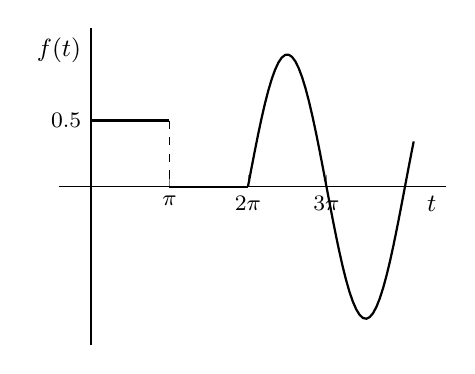
\begin{tikzpicture}
\begin{axis}[small,axis lines*=middle,xlabel={$t$},ylabel={$f(t)$},xlabel style={at={(current axis.right of origin)},anchor=north east},ylabel style={rotate=-90},ylabel style={at={(current axis.above origin)},anchor=north east},xtick={0,180,360,540},xticklabels={$0$,$\pi$,$2\pi$,$3\pi$},ytick={0.5},yticklabels={$0.5$}]
%function
\addplot[thick] plot coordinates {(0,0.5) (180,0.5)};
\addplot[dashed] plot coordinates {(180,0.5) (180,0)};
\addplot[thick] plot coordinates {(180,0) (360,0)};
\addplot[thick,domain=360:740,samples=50] {sin(x)};
\end{axis}
\end{tikzpicture}
\caption*{(ب) مثال \حوالہ{مثال_لاپلاس_عملی_الف} کا تفاعل۔}
\end{subfigure}%
\caption{مثال \حوالہ{مثال_لاپلاس_منتقلی_وقتی_محور_الف} اور مثال \حوالہ{مثال_لاپلاس_عملی_الف} کے تفاعل۔}
\label{شکل_مثال_لاپلاس_منتقلی_وقتی_محور_الف}
\end{figure}
\انتہا{مثال}
%======================
\ابتدا{مثال}\شناخت{مثال_لاپلاس_عملی_الف}
شکل \حوالہ{شکل_مثال_لاپلاس_منتقلی_وقتی_محور_الف}-ب میں درج ذیل تفاعل دکھایا گیا ہے۔اس کا لاپلاس بدل حاصل کریں۔
\begin{align*}
f(t)=
\begin{cases}
0.5 & 0<t<\pi\\
0&\pi<t<2\pi\\
\sin t&t>2\pi
\end{cases}
\end{align*}
حل:اکائی سیڑھی تفاعل کی مدد سے دیے گئے تفاعل کو لکھتے ہیں
\begin{align*}
f(t)=0.5u(t)-0.5u(t-\pi)+u(t-2\pi)\sin t
\end{align*}
جہاں \عددی{\sin(t-2\pi)=\sin t} کا استعمال کیا گیا ہے۔مساوات \حوالہ{مساوات_لاپلاس_اکائی_سیڑھی}، مساوات \حوالہ{مساوات_لاپلاس_منتقلی_وقت_صورت_الف} اور جدول \حوالہ{جدول_لاپلاس_بدل_الف} کی مدد سے لاپلاس بدل لکھتے ہیں۔
\begin{align*}
\Laplace(f)=\frac{0.5}{s}-\frac{0.5e^{-\pi s}}{s}+\frac{e^{-2\pi s}}{s^2+1}
\end{align*}
\انتہا{مثال}
%========================
\ابتدا{مثال}\شناخت{مثال_لاپلاس_سلسلہ_وار_دور_الف}\quad ایک عدد چکور موج پر \عددی{RC} دور کا رد عمل\\ 
مزاحمت اور برق گیر کا سلسلہ وار دور شکل میں دکھایا گیا ہے۔اس کو ایک عدد چکور موج \عددی{v(t)} مہیا کی جاتی ہے۔دور میں برقی رو \عددی{i(t)} دریافت کریں۔ شکل \حوالہ{شکل_مثال_لاپلاس_سلسلہ_وار_دور_الف} سے رجوع کریں۔
\begin{figure}
\centering
\begin{subfigure}{0.4\textwidth}
\begin{tikzpicture}
\draw(0,0) to [american voltage source,l={$v(t)$}]++(0,\y) to [resistor,l={$R$},i={$i(t)$}]++(\x,0) to [capacitor,l={$C$}]++(0,-\y) to [short]++(-\x,0);
\end{tikzpicture}
\end{subfigure}%
\begin{subfigure}{0.6\textwidth}
\centering
\begin{tikzpicture}
\begin{axis}[small,axis lines*=middle, xtick={1,2},xticklabels={$a$,$b$},ytick={1},yticklabels={$V_0$},xlabel={$t$},ylabel={$v(t)$},xlabel style={at={(current axis.right of origin)},anchor=north east},ylabel style={at={(current axis.above origin)},anchor=north east},ylabel style={rotate=-90},ymax=1.5]
\addplot[thick] plot coordinates {(0,0) (1,0)};
\addplot[dashed] plot coordinates {(1,0) (1,1)};
\addplot[thick] plot coordinates {(1,1) (2,1)};
\addplot[dashed] plot coordinates {(2,1) (2,0) };
\addplot[thick] plot coordinates {(2,0) (3,0) };
\end{axis}
\end{tikzpicture}
\end{subfigure}%
\caption{مثال \حوالہ{مثال_لاپلاس_سلسلہ_وار_دور_الف} کا دور اور داخلی دباو۔}
\label{شکل_مثال_لاپلاس_سلسلہ_وار_دور_الف}
\end{figure}

حل:کرخوف مساوات دباو سے 
\begin{align*}
i(t)R+\frac{1}{C}\int_{0}^{t} i(\tau)\dif \tau=v(t)
\end{align*}
لکھ سکتے ہیں جہاں داخلی دباو کو دو عدد اکائی سیڑھی تفاعل کی مدد سے 
\begin{align*}
v(t)=V_0(u(t-a)-u(t-b))
\end{align*}
لکھا جا سکتا ہے۔مساوات \حوالہ{مساوات_لاپلاس_اکائی_سیڑھی} اور مسئلہ \عددی{مساوات_لاپلاس_تکمل_کا_بدل} استعمال کرتے ہوئے  ضمنی مساوات لکھتے ہیں
\begin{align*}
I(s)R+\frac{I(s)}{sC}=\frac{V_0}{s}[e^{-as}-e^{-bs}]
\end{align*}
جس کا حل درج ذیل ہے۔
\begin{align*}
I(s)=\left(\frac{\frac{V_0}{R}}{s+\frac{1}{RC}}\right)[e^{-as}-e^{-bs}]
\end{align*}
اب ہم جدول \حوالہ{جدول_لاپلاس_بدل_الف} سے جانتے ہیں کہ
\begin{align*}
\Laplace^{-1}\left(\frac{\frac{V_0}{R}}{s+\frac{1}{RC}}\right)=\Laplace^{-1}[F(s)]=\frac{V_0}{R}e^{-\frac{t}{RC}}
\end{align*}
کے برابر ہے لہٰذا اصل حل مسئلہ \حوالہ{مسئلہ_لاپلاس_وقتی_محور_منتقلی} کے تحت  درج ذیل ہو گا
\begin{align*}
i(t)&=\Laplace^{-1}(I)=\Laplace^{-1}[e^{-as}F(s)]-\Laplace^{-1}[e^{-bs}F(s)]\\
&=\frac{V_0}{R}[e^{-\frac{(t-a)}{RC}}u(t-a)-e^{-\frac{(t-b)}{RC}}u(t-b)]
\end{align*}
جس کو یوں
\begin{align*}
i(t)=
\begin{cases}
0&t<a\\
K_1e^{-\frac{t}{RC}}& a<t<b\\
(K_1-K_2)e^{-\frac{t}{RC}} & t>b
\end{cases}
\end{align*}
بھی لکھا جا سکتا ہے جہاں \عددی{K_1=\frac{V_0}{R}e^{\frac{a}{RC}}} اور \عددی{K_2=\frac{V_0}{R}e^{\frac{b}{RC}}} ہیں۔ برقی رو \عددی{i(t)} کو شکل \حوالہ{شکل_مثال_لاپلاس_سلسلہ_وار_دور_الف_رو} میں دکھایا گیا ہے۔
\begin{figure}
\centering
\begin{tikzpicture}
\begin{axis}[small,axis lines*=middle,xlabel={$t$},ylabel={$i(t)$},xlabel style={at={(current axis.right of origin)},anchor=north},ylabel style={rotate=-90},ylabel style={at={(current axis.above origin)},anchor=north east},xtick={1,2},xticklabels={$a$,$b$},ytick={1},yticklabels={$\frac{V_0}{R}$},ymax=1.5]
\addplot[] plot coordinates {(0,0) (1,0)};
\addplot[domain=1:2]{e^1*e^(-x)};
\addplot[domain=2:4]{(e^1-e^2)*e^(-x)};
\addplot[] plot coordinates {(1,0) (1,1)};
\addplot[] plot coordinates {(2,0.367879) (2,-0.63212)};
\end{axis}
\end{tikzpicture}
\caption{مثال \حوالہ{مثال_لاپلاس_سلسلہ_وار_دور_الف} کی رو \عددی{i(t)}}
\label{شکل_مثال_لاپلاس_سلسلہ_وار_دور_الف_رو}
\end{figure}
\انتہا{مثال}
%===============================
\ابتدا{مثال}\شناخت{مثال_لاپلاس_بلا_تقصیر_اکائی}\quad بلا تقصیر نظام کا رد عمل۔ ایک عدد چکور داخلی موج\\
درج ذیل ابتدائی قیمت مسئلہ حل کریں جہاں \عددی{r(t)} کو شکل \حوالہ{مثال_لاپلاس_تقصیر_اکائی} میں دکھایا گیا ہے۔
\begin{align*}
y''+4y=r(t),\quad \quad y(0)=0, \, y'(0)=0
\end{align*}
حل:داخلی جبری قوت کو \عددی{r(t)=2[u(t)-u(t-1)]} لکھا جا سکتا ہے۔دیے گئے ابتدائی قیمت مسئلے  سے ضمنی مساوات لکھتے ہیں
\begin{align*}
s^2Y+4Y=\frac{2}{s}(1-e^{-s})
\end{align*} 
جس کا حل درج ذیل ہے۔
\begin{align*}
Y=\frac{2}{s(s^2+4)}(1-e^{-s})
\end{align*}
اب جدول \حوالہ{جدول_لاپلاس_بدل_الف} کے تحت \عددی{\Laplace^{-1}(\tfrac{2}{s^2+4})=\sin 2t} ہے  لہٰذا مساوات \حوالہ{مساوات_لاپلاس_تکمل_کا_بدل_جڑواں} استعمال کرتے ہوئے درج ذیل لکھا جا سکتا ہے۔
\begin{align*}
\Laplace^{-1}\left[\frac{2}{s(s^2+4)}\right]=\int_{0}^{t}\sin 2\tau \dif \tau=\frac{1}{2}(1-\cos 2t)
\end{align*}
اب مسئلہ \حوالہ{مسئلہ_لاپلاس_وقتی_محور_منتقلی} زیر استعمال لاتے ہوئے اصل جواب لکھتے ہیں
\begin{align*}
y(t)=\frac{1}{2}[1-\cos 2t]-\frac{1}{2}[1-\cos 2(t-1)]u(t-1)
\end{align*}
جس کو درج ذیل بھی لکھا جا سکتا ہے۔ہم دیکھتے ہیں کہ رد عمل دو مختلف ہارمونی ارتعاش کا مجموعہ ہے۔
\begin{align*}
y(t)=
\begin{cases}
\frac{1}{2}[1-\cos 2t] & 0<t<1\\[0.5ex]
\frac{1}{2}[\cos 2(t-1)-\cos 2t]& t>1
\end{cases}
\end{align*}
%
\begin{figure}
\centering
\begin{tikzpicture}
\begin{axis}[small,axis lines*=middle, xlabel={$t$}, ylabel={$r(t)$},xtick={1},xticklabels={$1$},ytick={1},yticklabels={$2$},xlabel style={at={(current axis.right of origin)},anchor=north east},ylabel style={rotate=-90},ylabel style={at={(current axis.above origin)},anchor=north east},ymax=1.5]
\addplot[thick] plot coordinates {(0,1) (1,1) (1,0) (3,0)};
\end{axis}
\end{tikzpicture}
\caption{مثال \حوالہ{مثال_لاپلاس_بلا_تقصیر_اکائی} اور مثال \حوالہ{مثال_لاپلاس_تقصیر_اکائی} کا داخلی تفاعل۔}
\label{شکل_مثال_لاپلاس_تقصیر_اکائی}
\end{figure}
\انتہا{مثال}
%================================
\ابتدا{مثال}\شناخت{مثال_لاپلاس_تقصیر_اکائی}\quad قصری نظام کا رد عمل۔ ایک عدد چکور موج\\
درج ذیل قصری ابتدائی قیمت مسئلے کو حل کریں جہاں \عددی{r(t)} کو شکل \حوالہ{شکل_مثال_لاپلاس_تقصیر_اکائی} میں دکھایا گیا ہے۔
\begin{align*}
y''+4y'+3y=r(t) \quad \quad y(0)=0, \, y'(0)=0
\end{align*}
حل:ضمنی مساوات لکھ کر
\begin{align*}
s^2Y+4sY+3Y=\frac{2}{s}(1-e^{-s})
\end{align*}
حل کرتے ہوئے درج ذیل ملتا ہے۔
\begin{align*}
Y=\frac{2}{s(s+1)(s+3)}(1-e^{-s})
\end{align*}
\عددی{F(s)=\tfrac{2}{s(s+1)(s+3)}} کا جزوی کسری پھیلاو 
\begin{align*}
F(s)=\frac{2}{3s}+\frac{1}{3(s+3)}-\frac{1}{s+1}
\end{align*}
  ہے لہٰذا
\begin{align*}
f(t)=\Laplace^{-1}(F)=\frac{2}{3}+\frac{e^{-3t}}{3}-e^{-t}
\end{align*}
ہو گا۔یوں مسئلہ \حوالہ{مسئلہ_لاپلاس_وقتی_محور_منتقلی} کی مدد سے درج ذیل لکھا جا سکتا ہے۔
\begin{align*}
\Laplace^{-1}(Fe^{-s})=f(t-1)u(t-1)=
\begin{cases}
0& 0<t<1\\
\frac{2}{3}+\frac{e^{-3(t-1)}}{3}-e^{-(t-1)} & t>1
\end{cases}
\end{align*}
ان نتائج کو استعمال کرتے ہوئے اصل حل لکھتے ہیں۔
\begin{align*}
y(t)=\Laplace^{-1}(Y)=f(t)-f(t-1)u(t-1)=
\begin{cases}
\frac{2}{3}+\frac{e^{-3t}}{3}-e^{-t} & 0<t<1\\
(1-e^3)\frac{e^{-3t}}{3}-(1-e)e^{-t}& t>1
\end{cases}
\end{align*}
\انتہا{مثال}
%=======================================
\ابتدا{مثال}\شناخت{مثال_لاپلاس_تکمل_الف}
شکل \حوالہ{شکل_مثال_لاپلاس_تکمل_الف}-الف میں تفاعل \عددی{f(t)} اور شکل-ب میں اس کا تکمل دکھایا گیا ہے۔\عددی{f(t)} کے بدل سے  شکل-ب کا لاپلاس بدل حاصل کریں۔
\begin{figure}
\centering
\begin{subfigure}{0.5\textwidth}
\centering
\begin{tikzpicture}
%axis
\draw(0,0)--(0,1.5)node[left]{$f$};
\draw(0,0)--(4,0)node[right]{$t$};
%function
\draw[thick](0,0)--(1,0)node[below]{$a$}++(0,1)--++(2,0)++(0,-1)node[below]{$b$}--(4,0);
\draw[dashed] (1,0)--++(0,1)++(2,0)--++(0,-1);
\draw(0,1)--++(-0.1,0)node[left]{$1$};
\draw(2,-0.75)node[]{(الف)};
\end{tikzpicture}
\end{subfigure}%
\begin{subfigure}{0.5\textwidth}
\centering
\begin{tikzpicture}
%axis
\draw(0,0)--(0,1.5);
\draw(0,0)--(4,0)node[right]{$t$};
%function
\draw[thick](0,0)--(1,0)node[below]{$a$}--++(2,1)--++(1,0);
\draw(0,1)--++(-0.1,0)node[left]{$(b-a)$};
\draw(3,0)--++(0,-0.1)node[below]{$b$};
\draw(2,-0.75)node[]{(ب)};
\end{tikzpicture}
\end{subfigure}%
\caption{مثال \حوالہ{مثال_لاپلاس_تکمل_الف} کے اشکال۔}
\label{شکل_مثال_لاپلاس_تکمل_الف}
\end{figure} 

جواب:شکل \حوالہ{شکل_مثال_لاپلاس_تکمل_الف}-الف کا لاپلاس بدل \عددی{F=\tfrac{1}{s}(e^{-as}-e^{-bs})} ہے لہٰذا شکل-ب کا بدل
 \عددی{\tfrac{F}{s}=\tfrac{e^{-as}-e^{-bs}}{s^2}} ہو گا۔
\انتہا{مثال}
%=================================

\حصہء{سوالات}
سوال \حوالہ{سوال_لاپلاس_قوت_نمائی_الف} تا سوال \حوالہ{سوال_لاپلاس_قوت_نمائی_ب} کے لاپلاس بدل دریافت کریں۔

%==================
\ابتدا{سوال}\شناخت{سوال_لاپلاس_قوت_نمائی_الف} \quad
$e^{-3t}\sin 4t$\\
جواب:\عددی{\tfrac{4}{(s+3)^2+16}}
\انتہا{سوال}
%==================
\ابتدا{سوال}\quad
$e^{-t}\cos (\omega t-\theta)$\\
جواب:\عددی{\tfrac{(s+1)\cos \theta+\omega \sin \theta}{(s+1)^2+\omega^2}}
\انتہا{سوال}
%======================
\ابتدا{سوال}\quad
$e^{-at}(A\sin \omega t+B\cos \omega t)$\\
جواب:\عددی{\tfrac{\omega A+(s+a)B}{(s+a)^2+\omega^2}}
\انتہا{سوال}
%=====================
\ابتدا{سوال}\شناخت{سوال_لاپلاس_قوت_نمائی_ب}\quad
$e^{2t}(3t-4t^2)$\\
جواب:\عددی{\tfrac{3}{(s-2)^2}-\tfrac{8}{(s-2)^3}}
\انتہا{سوال}
%=====================
سوال \حوالہ{سوال_لاپلاس_قوت_نمائی_پ} تا سوال \حوالہ{سوال_لاپلاس_قوت_نمائی_ت} میں  بذلولی سائن اور بذلولی کوسائن کو قوت نمائی تفاعل کی صورت میں لکھ کر لاپلاس بدل حاصل کریں۔

%===============
\ابتدا{سوال}\شناخت{سوال_لاپلاس_قوت_نمائی_پ}\quad
$e^{-at}\sinh \omega t$\\
جواب:\عددی{\tfrac{\omega}{(s+a)^2-\omega^2}}
\انتہا{سوال}
%====================
\ابتدا{سوال}\quad
$\sinh at \sin a t$\\
جواب:\عددی{\tfrac{2a^2s}{s^4+4a^4}}
\انتہا{سوال}
%=====================
\ابتدا{سوال}\quad
$\sinh at\sin \omega t$\\
جواب:\عددی{\tfrac{\omega}{2[(s-a)^2+\omega^2]}-\tfrac{\omega}{2[(s+a)^2+\omega^2]}}
\انتہا{سوال}
%=========================
\ابتدا{سوال}\شناخت{سوال_لاپلاس_قوت_نمائی_ت}\quad
$t\cosh at$\\
جواب:\عددی{\tfrac{1}{2(s-a)^2}+\tfrac{1}{2(s+a)^2}}
\انتہا{سوال}
%=================
سوال \حوالہ{سوال_لاپلاس_الٹ_قوت_نمائی_الف} تا سوال \حوالہ{سوال_لاپلاس_الٹ_قوت_نمائی_ب} میں \عددی{\Laplace^{-1}} دریافت کریں۔

%===================
\ابتدا{سوال}\شناخت{سوال_لاپلاس_الٹ_قوت_نمائی_الف}\quad
$\frac{s+4}{(s+1)^2+9}$\\
جواب:\عددی{e^{-t}(\cos 3t+\sin 3t)}
\انتہا{سوال}
%===================
\ابتدا{سوال}\quad
$\frac{s-2}{s^2+4s+8}$\\
جواب:\عددی{e^{-2t}(\cos 2t-2\sin 2t)}
\انتہا{سوال}
%======================
\ابتدا{سوال}\quad
$\frac{2}{(s+1)^3}-\frac{6}{(s+1)^4}$\\
جواب:\عددی{e^{-t}(t^2+t^3)}
\انتہا{سوال}
%========================
\ابتدا{سوال}\شناخت{سوال_لاپلاس_الٹ_قوت_نمائی_ب}\quad
$\frac{as+b}{(s-c)^2+\omega}$\\
جواب:\عددی{e^{ct}[\frac{(ac+b)}{\omega}\sin \omega t+a\cos \omega t]}
\انتہا{سوال}
%======================

سوال \حوالہ{سوال_لاپلاس_ابتدائی_قیمت_الف} تا سوال \حوالہ{سوال_لاپلاس_ابتدائی_قیمت_ب} ابتدائی قیمت مسئلے ہیں۔انہیں لاپلاس بدل کی استعمال سے حل کریں۔

%================
\ابتدا{سوال}\شناخت{سوال_لاپلاس_ابتدائی_قیمت_الف}\quad
$y''+2y'+10y=0,\quad \quad y(0)=-2, \, y'(0)=1$\\
جواب:\عددی{y=-e^{-t}(2\cos 3t+\tfrac{1}{3}\sin 3t)}
\انتہا{سوال}
%=====================
\ابتدا{سوال}\quad
$y''-6y'+9y=0,\quad \quad y(0)=1, \, y'(0)=2$\\
جواب:\عددی{y=(1-t)e^{3t}}
\انتہا{سوال}
%=======================
\ابتدا{سوال}\quad
$y''-2y'+5y=0,\quad \quad y(0)=-1, \, y'(0)=1$\\
جواب:\عددی{y=e^t(\sin 2t-\cos 2t)}
\انتہا{سوال}
%========================
\ابتدا{سوال}\شناخت{سوال_لاپلاس_ابتدائی_قیمت_ب}\quad
$y''+10y'+25=0, \quad \quad y(0)=2, \, y'(0)=-1$\\
جواب:\عددی{y=(9t+2)e^{-5t}}
\انتہا{سوال}
%========================

اکائی سیڑھی تفاعل استعمال کرتے ہوئے سوال \حوالہ{سوال_لاپلاس_سیڑھی_الف} تا سوال \حوالہ{سوال_لاپلاس_سیڑھی_ث} میں دیے گئے خطوط کو لکھ کر ان کا لاپلاس بدل حاصل کریں۔

%=============
\ابتدا{سوال}\شناخت{سوال_لاپلاس_سیڑھی_الف}
شکل \حوالہ{شکل_سوال_لاپلاس_سیڑھی_الف}-الف میں دکھائے گیے خط بقایا تمام \عددی{t} پر صفر کے برابر ہے۔
\begin{figure}
\centering
\begin{subfigure}{0.5\textwidth}
\centering
\begin{tikzpicture}
%axis
\draw(0,-1)--(0,1);
\draw(0,0)--++(4,0)node[below right]{$t$};
%wave
\draw[thick](0,0.75)node[left]{$2$}--++(1,0)++(0,-1.25)--++(1,0)++(0,0.5)--(4,0);
\draw[dashed](1,0.75)--++(0,-1.25)++(1,0)--++(0,0.5);
\draw(0,-0.5)--++(-0.1,0)node[left]{$-1$};
\foreach \x in {0.5,1,1.5,2,2.5,3,3.5}{\draw (\x,0)--++(0,-0.1);}
\draw(1.5,0)node[above]{$3$};
\draw(3,0)node[above]{$6$};
\draw(2,-0.75)node{(الف)};
\end{tikzpicture}
\end{subfigure}%
\begin{subfigure}{0.5\textwidth}
\centering
\begin{tikzpicture}
%axis
\draw(0,-1)--(0,1);
\draw(0,0)--++(3.25,0)node[below right]{$t$};
%wave
\draw[thick](0,0.5)node[left]{$1$}--++(0.5,0)++(0,-0.5)--++(0.5,0)++(0,0.5)--++(0.5,0)++(0,-0.5)--++(0.5,0)++(0,0.5)--++(0.5,0)++(0,-0.5)--++(0.5,0)++(0,0.5)--++(0.25,0);
\foreach \x in {0.5,1,1.5,2,2.5,3}{\draw[dashed](\x,0)--++(0,0.5);}
\foreach \x in {0.5,1,1.5,2,2.5,3}{\draw (\x,0)--++(0,-0.1);}
\foreach \x/\y in {1/2,2/4,3/6} {\draw(\x,0)node[below]{$\y$};}
\draw(2,-0.75)node{(ب)};
\end{tikzpicture}
\end{subfigure}%
\caption{سوال \حوالہ{سوال_لاپلاس_سیڑھی_الف} اور سوال \حوالہ{سوال_لاپلاس_سیڑھی_ب} کے اشکال۔}
\label{شکل_سوال_لاپلاس_سیڑھی_الف}
\end{figure}

جواب:\عددی{\tfrac{1}{s}(2-3e^{-2s}+e^{-4s})}
\انتہا{سوال}
%==================
\ابتدا{سوال}\شناخت{سوال_لاپلاس_سیڑھی_ب}
شکل \حوالہ{شکل_سوال_لاپلاس_سیڑھی_الف}-ب مسلسل موج ہے۔

جواب:
\begin{align*}
f(t)&=u(t)-u(t-1)+u(t-2)-u(t-3)+u(t-4)-u(t-5)+-\cdots\\
\Laplace(f)&=\frac{1}{s}(1-e^{-s}+e^{-2s}-e^{-3s}+e^{-4s}-e^{-5s}+-\cdots)\\
&=\frac{1}{s}\left[\frac{1-(-e^{-s})^n}{1+e^{-s}}\right]=\frac{1}{s(1+e^{-s})}\quad 
 \text{\RL{\عددی{n \to \infty} ، \عددی{s>0} پر \عددی{e^{-sn} \to 0} ہو گا۔}}
\end{align*}
\انتہا{سوال}
%=========================
\ابتدا{سوال}\شناخت{سوال_لاپلاس_سیڑھی_پ}
شکل \حوالہ{شکل_سوال_لاپلاس_سیڑھی_پ}-الف مسلسل موج ہے۔
\begin{figure}
\centering
\begin{subfigure}{0.5\textwidth}
\centering
\begin{tikzpicture}
%axis
\draw(0,-1)--(0,1);
\draw(0,0)--++(3.25,0)node[below right]{$t$};
%wave
\draw[thick](0,0.5)node[left]{$1$}--++(0.5,0)++(0,-1)--++(0.5,0)++(0,1)--++(0.5,0)++(0,-1)--++(0.5,0)++(0,1)--++(0.5,0)++(0,-1)--++(0.5,0)++(0,1)--++(0.25,0);
\foreach \x in {0.5,1,1.5,2,2.5,3}{\draw[dashed](\x,-0.5)--++(0,1);}
\foreach \x in {0.5,1,1.5,2,2.5,3}{\draw (\x,0)--++(0,-0.1);}
\foreach \x/\y in {1/2,2/4} {\draw(\x,0)node[below right]{$\y$};}
\draw(2,-0.75)node{(الف)};
\end{tikzpicture}
\end{subfigure}%
\begin{subfigure}{0.5\textwidth}
\centering
\begin{tikzpicture}
%axis
\draw(0,0)--(0,2);
\draw(0,0)--++(3.25,0)node[below right]{$t$};
%wave
\draw[thick](0,0)--++(0,0.5)--++(1,0)--++(0,0.5)--++(1,0)--++(0,0.5)--++(1,0)--++(0,0.5)--++(0.25,0);
\foreach \x in {1,2,3}{\draw (\x,0)--++(0,-0.1);}
\foreach \x/\y in {1/1,2/2,3/3} {\draw(\x,0)node[below]{$\y$};}
\foreach \y/\t in {0.5/1,1/2,1.5/3}{\draw (0,\y)--++(-0.1,0)node[left]{$\t$};}
\draw(2,-0.75)node{(ب)};
\end{tikzpicture}
\end{subfigure}%
\caption{سوال \حوالہ{سوال_لاپلاس_سیڑھی_پ} اور سوال \حوالہ{سوال_لاپلاس_سیڑھی_ت} کے اشکال۔}
\label{شکل_سوال_لاپلاس_سیڑھی_پ}
\end{figure}

جواب:
\begin{align*}
f(t)&=u(t)-2u(t-1)+2u(t-2)-2u(t-3)+2u(t-4)-2u(t-5)+-\cdots\\
\Laplace(f)&=\frac{1}{s}-\frac{2e^{-s}}{s}+\frac{2e^{-2s}}{s}-\frac{2e^{-3s}}{s}+\frac{2e^{-4s}}{s}-\frac{2e^{-5s}}{s}+-\cdots\\
&=-\frac{1}{s}+\frac{2}{s}-\frac{2e^{-s}}{s}+\frac{2e^{-2s}}{s}-\frac{2e^{-3s}}{s}+\frac{2e^{-4s}}{s}-+\cdots=-\frac{1}{s}+\frac{2}{s(1+e^{-s})}
\end{align*}
\انتہا{سوال}
%====================
\ابتدا{سوال}\شناخت{سوال_لاپلاس_سیڑھی_ت}
شکل \حوالہ{شکل_سوال_لاپلاس_سیڑھی_پ}-ب مسلسل موج ہے۔

جواب:
\begin{align*}
f(t)&=u(t)+u(t-1)+u(t-2)+u(t-3)+u(t-4)+\cdots\\
\Laplace(f)&=\frac{1}{s}+\frac{e^{-s}}{s}+\frac{e^{-2s}}{s}+\frac{e^{-3s}}{s}+\cdots=\frac{1}{s(1-e^{-s})}
\end{align*}
\انتہا{سوال}
%==========================
%=========================
\ابتدا{سوال}\شناخت{سوال_لاپلاس_سیڑھی_ٹ}
شکل \حوالہ{شکل_سوال_لاپلاس_سیڑھی_ٹ}-الف مسلسل موج ہے۔
\begin{figure}
\centering
\begin{subfigure}{0.5\textwidth}
\centering
\begin{tikzpicture}
%axis
\draw(0,0)--(0,2);
\draw(0,0)--++(3.25,0)node[below right]{$t$};
%wave
\draw[thick](0,0)--++(1,0)--++(0,0.5)--++(1,0)--++(0,0.5)--++(1,0)--++(0,0.5)--++(0.25,0);
\foreach \x in {1,2,3}{\draw (\x,0)--++(0,-0.1);}
\foreach \x/\y in {1/1,2/2,3/3} {\draw(\x,0)node[below]{$\y$};}
\foreach \y/\t in {0.5/1,1/2,1.5/3}{\draw (0,\y)--++(-0.1,0)node[left]{$\t$};}
\draw(2,-0.75)node{(الف)};
\end{tikzpicture}
\end{subfigure}%
\begin{subfigure}{0.5\textwidth}
\centering
\begin{tikzpicture}
%axis
\draw(0,0)--(0,2);
\draw(0,0)--++(3.25,0)node[below right]{$t$};
%wave
\draw[thick](0,0)--++(0,0.5)--++(1,0)--++(0,0.5)--++(1,0)--++(0,-0.5)--++(1,0)--++(0,-0.5)--++(0.25,0);
\foreach \x in {1,2,3}{\draw (\x,0)--++(0,-0.1);}
\foreach \x/\y in {1/1,2/2,3/3} {\draw(\x,0)node[below]{$\y$};}
\foreach \y/\t in {0.5/1,1/2,1.5/3}{\draw (0,\y)--++(-0.1,0)node[left]{$\t$};}
\draw(2,-0.75)node{(ب)};
\end{tikzpicture}
\end{subfigure}%
\caption{سوال \حوالہ{سوال_لاپلاس_سیڑھی_ٹ} اور سوال \حوالہ{سوال_لاپلاس_سیڑھی_ث} کے اشکال۔}
\label{شکل_سوال_لاپلاس_سیڑھی_ٹ}
\end{figure}

جواب:
\begin{align*}
f(t)&=u(t-1)+u(t-2)+u(t-3)+u(t-4)+\cdots\\
\Laplace(f)&=\frac{e^{-s}}{s}+\frac{e^{-2s}}{s}+\frac{e^{-3s}}{s}+\cdots=\frac{e^{-s}}{s(1-e^{-s})}
\end{align*}
\انتہا{سوال}
%====================
\ابتدا{سوال}\شناخت{سوال_لاپلاس_سیڑھی_ث}
شکل \حوالہ{شکل_سوال_لاپلاس_سیڑھی_ٹ}-ب غیر مسلسل موج ہے۔بقایا تمام \عددی{t} پر موج صفر کے برابر ہے۔

جواب:\عددی{\tfrac{1}{s}(1+e^{-s}-e^{-2s}-e^{-3s})}
\انتہا{سوال}
%=======================
سوال \حوالہ{سوال_لاپلاس_الٹ_بدل_الف} تا سوال \حوالہ{سوال_لاپلاس_الٹ_بدل_ب} میں الٹ لاپلاس بدل حاصل کریں۔

%===============
\ابتدا{سوال}\شناخت{سوال_لاپلاس_الٹ_بدل_الف}\quad
$\frac{e^{-2s}-e^{-3s}}{s}$\\
جواب:\عددی{f=u(t-2)-u(t-3)} یعنی \عددی{2<t<3} کے لئے \عددی{f=1} ہے جبکہ بقایا اوقات \عددی{f=0} ہے۔
\انتہا{سوال}
%=============================
\ابتدا{سوال}\quad
$\frac{e^{-s}}{s^2}$\\
جواب:\عددی{(t-1)u(t-1)}
\انتہا{سوال}
%=========================
\ابتدا{سوال}\quad
$\frac{e^{-s}+2e^{-2s}-4e^{-3s}}{s^2}$\\
جواب:\عددی{t<1}، \عددی{1<t<2}، \عددی{2<t<3} اور \عددی{3<t} پر \عددی{f=0}، \عددی{f=t-1}، \عددی{f=3t-5} اور \عددی{f=-t+11} ہیں۔
\انتہا{سوال}
%==============================
\ابتدا{سوال}\شناخت{سوال_لاپلاس_الٹ_بدل_ب}\quad
$\frac{6(e^{-2s}-e^{-3s})}{s^3}$\\
جواب:\عددی{t<2}، \عددی{2<t<3} اور \عددی{3<t} کے لئے \عددی{f=0}، \عددی{f=(t-2)^2} اور \عددی{f=2t-5} ہے۔
\انتہا{سوال}
%===========================
 سوال \حوالہ{سوال_لاپلاس_بدل_اکائی_تفاعل_الف} تا سوال \حوالہ{سوال_لاپلاس_بدل_اکائی_تفاعل_ب}  کے لاپلاس بدل حاصل کریں۔

%=============
\ابتدا{سوال}\شناخت{سوال_لاپلاس_بدل_اکائی_تفاعل_الف}\quad
$(t-3)u(t-3)$\\
جواب:\عددی{\frac{e^{-3s}}{s^2}}
\انتہا{سوال}
%======================
\ابتدا{سوال}\quad
$tu(t)$\\
جواب:\عددی{\tfrac{1}{s^2}}
\انتہا{سوال}
%=======================
\ابتدا{سوال}\quad
$u(t-\pi)\sin t$\\
جواب:\عددی{\tfrac{1+e^{-\pi s}}{s^2+1}}
\انتہا{سوال}
%======================
\ابتدا{سوال}\quad
$u(t-\tfrac{2\pi}{\omega})\sin \omega t$\\
جواب:\عددی{\tfrac{\omega(1-e^{-\tfrac{2\pi s}{\omega}})}{s^2+\omega^2}}
\انتہا{سوال}
%======================
\ابتدا{سوال}\شناخت{سوال_لاپلاس_بدل_اکائی_تفاعل_ب}\quad
$t^2u(t-1)$\\
جواب:\عددی{\tfrac{(s^2+2s+2)e^{-s}}{s^3}}
\انتہا{سوال}
%=========================
 سوال \حوالہ{سوال_لاپلاس_وقفہ_الف} تا سوال \حوالہ{سوال_لاپلاس_وقفہ_ب} کے تفاعل دیے گئے وقفے کے باہر صفر کے برابر ہیں۔ ان کا لاپلاس بدل حاصل کریں۔ 

%==============
\ابتدا{سوال}\شناخت{سوال_لاپلاس_وقفہ_الف}\quad
$A\sin \omega t\quad \quad (0<t<\tfrac{\pi}{\omega})$\\
جواب:\عددی{\tfrac{A}{s^2+\omega^2}(1+e^{-\tfrac{\pi s}{\omega}})}

\انتہا{سوال}
%====================
\ابتدا{سوال}\quad
$A\cos \omega t \quad \quad (0<t<\tfrac{\pi}{2\omega})$\\
جواب:\عددی{\tfrac{A}{s^2+\omega^2}(s+\omega e^{-\tfrac{\pi s}{2\omega}})}
\انتہا{سوال}
%====================
\ابتدا{سوال}\شناخت{سوال_لاپلاس_وقفہ_ب}\quad
$t^2\quad \quad (0<t<1)$\\
جواب:\عددی{\tfrac{2-(s^2+2s+2)e^{-s}}{s^3}}
\انتہا{سوال}
%=======================
سوال \حوالہ{سوال_لاپلاس_الٹ_حاصل_الف} تا سوال \حوالہ{سوال_لاپلاس_الٹ_حاصل_ب} کے الٹ لاپلاس بدل حاصل کریں۔

%====================
\ابتدا{سوال}\شناخت{سوال_لاپلاس_الٹ_حاصل_الف}\quad
$\tfrac{e^{-3s}}{s}$\\
جواب:\عددی{u(t-3)}
\انتہا{سوال}
%====================
\ابتدا{سوال}\quad
$\tfrac{e^{-4s}}{s^2}$\\
جواب:\عددی{(t-4)u(t-4)}
\انتہا{سوال}
%===================
\ابتدا{سوال}\quad
$\tfrac{e^{-3s}}{s-4}$\\
جواب:\عددی{e^{4(t-3)}u(t-3)}
\انتہا{سوال}
%=======================
\ابتدا{سوال}\quad
$\tfrac{\omega e^{-2s}}{s^2+\omega^2}$\\
جواب:\عددی{\sin [\omega (t-2)] u(t-2)}

\انتہا{سوال}
%=======================
\ابتدا{سوال}\quad
$\tfrac{1-e^{-2s}}{s^2+9}$\\
جواب:\عددی{\tfrac{1}{3}\sin 3t u(t)-\tfrac{1}{3}\sin [3(t-2)]u(t-2)}
\انتہا{سوال}
%==========================
\ابتدا{سوال}\شناخت{سوال_لاپلاس_الٹ_حاصل_ب}\quad
$\tfrac{e^{-\pi s}}{s^2+2s+2}$\\
جواب:وقفہ \عددی{t>\pi} پر تفاعل \عددی{f=-e^{(\pi -t)}\sin (t-\pi)u(t-\pi)} ہے۔بقایا اوقات تفاعل صفر کے برابر ہے۔
\انتہا{سوال}
%==========================
سوال \حوالہ{سوال_لاپلاس_امالہ_برق_گیر_الف} تا سوال \حوالہ{سوال_لاپلاس_امالہ_برق_گیر_ب} میں \عددی{L=\SI{1}{\henry}} اور \عددی{C=\SI{1}{\farad}} لیتے ہوئے برقی رو \عددی{i(t)} دریافت کریں۔داخلی دباو \عددی{v(t)} سوال میں دیا گیا ہے۔

\begin{figure}
\centering
\begin{tikzpicture}
\draw(0,0) to [american voltage source,l={$v(t)$}]++(0,\y) to [inductor,i={$i(t)$},l={$L$}]++(\x,0) to [capacitor,l={$C$}]++(0,-\y) to [short]++(-\x,0);
\end{tikzpicture}
\caption{سوال \حوالہ{سوال_لاپلاس_امالہ_برق_گیر_الف} تا سوال \حوالہ{سوال_لاپلاس_امالہ_برق_گیر_ب} کا دور۔}
\label{شکل_سوال_لاپلاس_امالہ_برق_گیر_الف}
\end{figure}

%===================
\ابتدا{سوال}\شناخت{سوال_لاپلاس_امالہ_برق_گیر_الف}
\عددی{0<t<a} داخلی دباو \عددی{v(t)=t} ہے۔ بقایا اوقات \عددی{v(t)=0} ہے۔

جواب:
\begin{align*}
Li'+\tfrac{1}{C}\int_{0}^{t}i\dif t=t[1-u(t-a)]=t-(t-a)u(t-a)-au(t-a)\\
i=
\begin{cases}
1-\cos t& 0<t<a\\
\cos(t-a)-a\sin(t-a)-\cos t & t>a
\end{cases}
\end{align*} 
\انتہا{سوال}
%=========================
\ابتدا{سوال}\شناخت{سوال_لاپلاس_امالہ_برق_گیر_ب}
\عددی{0<t<\pi} پر \عددی{v(t)=1-e^{-t}} ہے جبکہ بقایا اوقات \عددی{v(t)=0} ہے۔

جواب:
\begin{align*}
i=
\begin{cases}
\tfrac{1}{2}(e^{-t}-\cos t+\sin t) & 0<t<a\\
-\tfrac{1}{2}(1+e^{-\pi})\cos t+\tfrac{1}{2}(3-e^{-\pi})\sin t& t>\pi
\end{cases}
\end{align*}
\انتہا{سوال}
%==========================
\ابتدا{سوال}
ثابت کریں کہ اگر \عددی{\Laplace[f(t)]=F(s)} ہو تب \عددی{\Laplace[f(at)]=\tfrac{F(\tfrac{s}{a})}{a}} ہو گا۔اس کلیے کو استعمال کرتے ہوئے \عددی{\cos t} کے لاپلاس بدل سے \عددی{\cos \omega t} کا لاپلاس بدل حاصل کریں۔
\انتہا{سوال}
%=====================
\ابتدا{سوال}
ثابت کریں کہ مساوات \حوالہ{مساوات_لاپلاس_منتقلی_وقت_صورت_الف} سے درج ذیل لکھا جا سکتا ہے جو عملاً زیادہ بہتر صورت ہے۔
\begin{align}
e^{-as}\Laplace[f(t+a)]=\Laplace[f(t)u(t-a)]
\end{align}

جواب:نیا تفاعل \عددی{\tilde{f}(t)} جہاں \عددی{\tilde{f}(t)=f(t+a)} ہے زیر استعمال لاتے ہیں۔یوں \عددی{f(t)=\tilde{f}(t-a)} ہو گا۔یوں مساوات \حوالہ{مساوات_لاپلاس_منتقلی_وقت_صورت_الف} سے درج ذیل لکھنا ممکن ہے۔
\begin{align*}
\Laplace[f(t)u(t-a)]=\Laplace[\tilde{f}(t-a)u(t-a)]=e^{-as}\Laplace[\tilde{f}(t)]=e^{-as}\Laplace[f(t+a)]
\end{align*}
\انتہا{سوال}
%======================

\حصہ{ڈیراک ڈیلٹائی تفاعل۔ اکائی ضرب تفاعل۔ جزوی کسری پھیلاو}
الیکٹران کی کمیت کو نقطہ کمیت تصور کیا جا سکتا ہے۔اسی طرح اس کی برقی بار کو نقطہ بار تصور کیا جا سکتا ہے۔یوں کارتیسی محور کے مرکز پر موجود الیکٹران کی کمیت مرکز پر پائی جائے گی جبکہ مرکز سے ہٹ کر کسی بھی نقطے پر کمیت صفر کے برابر ہو گی۔نقطہ کمیت یا نقطہ بار کو \اصطلاح{ڈیراک ڈیلٹائی تفاعل}\فرہنگ{ڈیراک!ڈیلٹائی تفاعل}\حاشیہب{Dirac delta function}\فرہنگ{Dirac!delta function} سے ظاہر\حاشیہد{ماہر طبیعیات، پال اڈرین مارث ڈیراک [1902-1984] (جرمنی کے ارون روڈالف یوسف شروڈِنگر کے ساتھ مشترق) نوبل انعام یافتہ [1933] ، انگلستان کے رہائشی (جن کا تعلق سوئزرلینڈ سے تھا) نے  کوانٹم میکانیات میں کلیدی کردار ادا کیا۔} کیا جاتا ہے۔اسی طرح گیند کو بلے سے مارتے ہوئے یا بندوق سے گولی چلاتے وقت  انتہائی کم دورانیے کے لئے قوت عمل میں آتی ہے۔ایسی قوت کو بھی ڈیراک ڈیلٹائی تفاعل سے ظاہر کیا جاتا ہے۔

ایسی برقی یا میکانی قوت (یا عمل) جو انتہائی کم دورانیے کے لئے کار آمد ہو کو \اصطلاح{ڈیراک ڈیلٹائی تفاعل} سے ظاہر کرتے ہوئے  مسئلے کو لاپلاس بدل کی مدد سے نہایت عمدگی کے ساتھ حل کیا جا سکتا ہے۔

ڈیراک ڈیلٹائی تفاعل کو شکل \حوالہ{شکل_ڈائی_رک_ڈیلٹائی_تفاعل} کی مدد سے سمجھتے ہیں جس میں درج ذیل تفاعل دکھایا گیا ہے، جہاں  \عددی{k} مثبت اور چھوٹی قیمت ہے۔
\begin{align}\label{مساوات_لاپلاس_اکائی_ضرب_الف}
f_k(t-a)=
\begin{cases}
\frac{1}{k}& a-\tfrac{k}{2}<t<a+\tfrac{k}{2}\\
0 & \text{\RL{بقایا \عددی{t}}}
\end{cases}
\end{align}
%
\begin{figure}
\centering
\begin{tikzpicture}
\draw(-2,0)--(2,0)node[right]{$t$};
\draw[thick](-1.5,0)--++(1,0)--++(0,1.5)--++(1,0)--++(0,-1.5)--++(1,0);
\draw[stealth-stealth] (-0.75,0)--++(0,1.5)node[pos=0.5,fill=white]{$\frac{1}{k}$};
\draw[] (-0.5,1.5)++(-0.1,0)--++(-0.3,0);
\draw[stealth-stealth](-0.5,0.5)--++(1,0)node[pos=0.5,fill=white]{$k$};
\draw[stealth-] (0,1) to [out=30,in=180]++(1,0.5)node[right]{\RL{اکائی رقبہ}};
\draw(0,0)--++(0,-0.1)node[below]{$a$};
\draw[stealth-] (-0.5,0)++(0,-0.1) to [out=-90, in=0]++(-0.5,-0.5)node[left]{$a-\tfrac{k}{2}$};
\draw[stealth-] (0.5,0)++(0,-0.1) to [out=-90, in=180]++(0.5,-0.5)node[right]{$a+\tfrac{k}{2}$};
\end{tikzpicture}
\caption{ڈیراک ڈیلٹائی تفاعل۔}
\label{شکل_ڈائی_رک_ڈیلٹائی_تفاعل}
\end{figure}

یہ تفاعل کسی ایسی قوت کو ظاہر کر سکتی ہے جس کی مقدار \عددی{\tfrac{1}{k}}  ہو اور جو لمحہ \عددی{t=a-\tfrac{k}{2}} تا \عددی{t=a+\tfrac{k}{2}} عمل پیرا ہو۔ میکانیات میں ایسی قوت کا، لمحہ  \عددی{t=a-\tfrac{k}{2}} تا \عددی{t=a+\tfrac{k}{2}}، تکمل میکانی \اصطلاح{ضرب}\فرہنگ{ضرب}\حاشیہب{impulse}\فرہنگ{impulse} کہلاتی ہے۔برقی میدان میں ایسے برقی دباو کو برقی \اصطلاح{ضرب} کہا جاتا ہے۔ شکل \حوالہ{شکل_ڈائی_رک_ڈیلٹائی_تفاعل} میں \اصطلاح{ضرب} درج ذیل ہے۔
\begin{align}\label{مساوات_لاپلاس_اکائی_ضرب_ب}
I_k=\int_{0}^{\infty} f_k(t-a)\dif t=\int_{a-\tfrac{k}{2}}^{a+\tfrac{k}{2}}\frac{1}{k}\dif t=1
\end{align}

آئیں دیکھتے ہیں کہ \عددی{k} کی قیمت کم سے کم کرنے سے \اصطلاح{ضرب} کی قیمت پر کیا اثر پڑتا ہے۔ہم \عددی{f_k} کی قیمت کی حد \عددی{k \to 0 } پر حاصل کرتے ہیں جہاں \عددی{k>0} ہے۔اس حد کو \اصطلاح{ڈیراک ڈیلٹائی تفاعل} یا \اصطلاح{اکائی ضرب تفاعل}\فرہنگ{اکائی ضرب تفاعل}\فرہنگ{اکائی!ضرب}\حاشیہب{unit impulse function}\فرہنگ{unit!impulse} پکارا اور \عددی{\delta(t-a)} سے ظاہر کیا جاتا ہے۔
\begin{align}
\delta(t-a)=\lim_{k \to 0} f_k(t-a)
\end{align}
\عددی{\delta(t-a)} کو، علم الاحصاء میں سادہ تفاعل کی رسمی مطلب کے تحت تفاعل نہیں سمجھا جا سکتا ہے البتہ اسے \ترچھا{عمومی تفاعل}\حاشیہد{روسی ریاضی دان سرگی لووچ سوبولو [1908-1989] نے عمومی تفاعل کے نظریے کی بنیاد رکھی۔} کے تحت تفاعل سمجھا جا سکتا ہے۔یہ حقیقت سمجھنے کی خاطر ہم دیکھتے ہیں کہ \عددی{f_k} کا \عددی{I_k} اکائی \عددی{(1)} ہے لہٰذا  مساوات \حوالہ{مساوات_لاپلاس_اکائی_ضرب_الف} اور مساوات \حوالہ{مساوات_لاپلاس_اکائی_ضرب_ب} میں \عددی{k \to 0} پر کرنے سے درج ذیل حاصل ہو گا
\begin{align}
\delta(t-a)=
\begin{cases}
\infty& t=a\\
0& t\ne a
\end{cases}
\quad \quad \int_{0}^{\infty}\delta(t-a)\dif t=1
\end{align}
جبکہ علم الاحصاء کے تحت، ایسے تفاعل کا تکمل صفر کے برابر ہو گا جس کی قیمت، ماسوائے کسی ایک نقطہ پر، صفر کے برابر ہو۔ اس کے باوجود \اصطلاح{ضرب} تفاعل استعمال کرتے ہوئے، اپنی آسانی کی خاطر، ہم \عددی{\delta(t-a)} کو سادہ تفاعل تصور کرتے ہیں۔بالخصوص \عددی{\delta(t-a)} کی  \اصطلاح{چننے}\فرہنگ{چننا!خاصیت}\حاشیہب{sifting property}\فرہنگ{sifting property} کی خاصیت استعمال کرتے ہوئے  استمراری تفاعل \عددی{g(t)} کے لئے درج ذیل لکھا جا سکتا ہے۔
\begin{multline*}
\int_{0}^{\infty}g(t)\delta(t-a)\dif t=\int_{0}^{a_-}g(t)\delta(t-a)\dif t+\int_{a_-}^{a_+}g(t)\delta(t-a)\dif t\\
+\int_{a_+}^{\infty}g(t)\delta(t-a)\dif t
\end{multline*}
چونکہ \عددی{t \ne 0} پر \عددی{\delta(t-a)=0} ہے لہٰذا درج بالا دائیں ہاتھ پہلا اور تیسرا تکمل صفر کے برابر ہیں۔یوں
\begin{align}\label{مساوات_لاپلاس_اکائی_ضرب_چننے_کی_صلاحیت}
\int_{0}^{\infty}g(t)\delta(t-a)\dif t&=\int_{a_-}^{a_+} g(t)\delta(t-a)\dif t=g(a)\int_{a_-}^{a_+} \delta(t-a)\dif t=g(a)
\end{align}
حاصل ہوتا ہے۔نقطہ \عددی{a} لامتناہی کم وسعت کا ہو گا جس پر \عددی{g(t)} کی قیمت میں تبدیلی کو رد کیا جا سکتا ہے۔یوں اس نقطے  پر \عددی{g(t)} کی قیمت، مستقل مقدار \عددی{g(a)} ہو گی۔اس مستقل مقدار \عددی{g(a)} کو تکمل کے باہر لے جایا گیا ہے جبکہ \عددی{\delta(t-a)} کا تکمل اکائی کے برابر ہے۔

\عددی{\delta(t-a)} کا لاپلاس بدل حاصل کرنے کی خاطر ہم درج ذیل لکھتے ہیں
\begin{align*}
f_k(t-a)=\frac{1}{k}u[t-(a-\tfrac{k}{2})]-\frac{1}{k}u[t-(a+\tfrac{k}{2})]
\end{align*}
لہٰذا
\begin{align*}
\Laplace(f_k)&=\frac{e^{-(a-\tfrac{k}{2})s}}{ks}-\frac{e^{-(a+\tfrac{k}{2})s}}{ks}=e^{-as}\left(\frac{e^{\tfrac{ks}{2}}-e^{-\tfrac{ks}{2}}}{ks}\right)
\end{align*}
ہو گا۔اب \عددی{k \to 0} پر درج بالا \عددی{\Laplace[\delta(t-a)]} دے گا۔ہم \عددی{e^{\mp x}=1\mp x+\tfrac{x^2}{2!}\mp +\cdots} استعمال کرتے ہوئے  قوسین کو پھیلا کر لکھتے ہیں۔
\begin{align*}
\frac{e^{\tfrac{ks}{2}}-e^{-\tfrac{ks}{2}}}{ks}=\frac{(1+\tfrac{ks}{2}+\tfrac{(\tfrac{ks}{2})^2}{2!}+\cdots)-(1-\tfrac{ks}{2}+\tfrac{(\tfrac{ks}{2})^2}{2!}-\cdots)}{ks}=\frac{ks+\tfrac{1}{3}(\tfrac{ks}{2})^3+\cdots}{ks}
\end{align*}
یوں \عددی{k \to 0} پر قوسین کی حد درج ذیل ہو گی
\begin{align*}
\lim_{k \to 0} \frac{ks+\tfrac{1}{3}(\tfrac{ks}{2})^3+\cdots}{ks}=1
\end{align*}
لہٰذا ڈیراک ڈیلٹائی تفاعل کا لاپلاس بدل درج ذیل ہو گا۔
\begin{align}\label{مساوات_لاپلاس_اکائی_ضرب_کا_بدل}
\Laplace[\delta(t-a)]=e^{-as}
\end{align}
اکائی سیڑھی تفاعل اور اکائی ضرب تفاعل کے لاپلاس بدل جانتے ہوئے، آئیں اب سادہ تفرقی مساوات کو حل کرتے ہوئے لاپلاس بدل کی طاقت دیکھیں۔آپ مثال \حوالہ{مثال_لاپلاس_قصری_اسپرنگ_کمیت_الف}، مثال \حوالہ{مثال_لاپلاس_اسپرنگ_کمیت_اکائی_ضرب_الف} اور مثال \حوالہ{مثال_لاپلاس_بدل_نیم_موج} کو دیگر طریقوں سے حل کر کے تسلی کر سکتے ہیں کہ لاپلاس بدل کا طریقہ نہایت عمدہ ہے۔ 

%======================
\ابتدا{مثال}\شناخت{مثال_لاپلاس_قصری_اسپرنگ_کمیت_الف}
درج ذیل اسپرنگ اور کمیت کی قصری نظام (حصہ \حوالہ{حصہ_سادہ_دو_جبری_ارتعاش}) کا رد عمل، شکل \حوالہ{شکل_مثال_لاپلاس_قصری_اسپرنگ_کمیت_الف} میں دکھائے گئے، اکائی چکور جبری قوت کی صورت میں حاصل کریں۔  
\begin{align}
y''+4y'+3y=r(t)=u(t-1)-u(t-2)\quad \quad y(0)=0,\, y'(0)=0
\end{align}
%
\begin{figure}
\centering
\begin{tikzpicture}
\begin{axis}[small,axis lines*=middle, xlabel={$t$}, xlabel style={at={(current axis.right of origin)},anchor=north east},ylabel={$y(t)$},ylabel style={rotate=-90},ylabel style={at={(current axis.above origin)},anchor=north east},ymax=1.5,xmax=3.9,ytick={1},yticklabels={$1$}]
\addplot[] plot coordinates {(0,0) (1,0)};
\addplot[] plot coordinates {(1,1) (2,1)};
\addplot[] plot coordinates {(2,0) (3,0)};
\addplot[dashed] plot coordinates {(1,0) (1,1)};
\addplot[dashed] plot coordinates {(2,0) (2,1)};
%
\addplot[domain=1:2]{1/3-1/2*e^(-3*(x-1))+1/6*e^(-3*(x-1))};
\addplot[domain=2:4]{-1/2*e^(-3*(x-1))+1/6*e^(-3*(x-1))+1/2*e^(-3*(x-2))-1/6*e^(-3*(x-2))};
\end{axis}
\end{tikzpicture}
\caption{اسپرنگ اور کمیت کا قصری نظام (مثال \حوالہ{مثال_لاپلاس_قصری_اسپرنگ_کمیت_الف})۔}
\label{شکل_مثال_لاپلاس_قصری_اسپرنگ_کمیت_الف}
\end{figure}

حل:دیے گئے تفرقی مساوات سے ضمنی مساوات لکھتے ہیں۔ایسا مساوات \حوالہ{مساوات_لاپلاس_درجہ_اول_تفرق}، مساوات \حوالہ{مساوات_لاپلاس_درجہ_دوم_تفرق} اور مساوات \حوالہ{مساوات_لاپلاس_اکائی_سیڑھی} کی مدد سے کیا جائے گا۔
\begin{align*}
s^2Y+4sY+3Y=\frac{e^{-s}}{s}-\frac{e^{-2s}}{s}
\end{align*}
ضمنی مساوات کا حل
\begin{align*}
Y=\frac{1}{s(s^2+4s+3)}(e^{-s}-e^{-2s})=\frac{1}{s(s+1)(s+3)}(e^{-s}-e^{-2s})
\end{align*}
ہے جس کا جزوی کسری پھیلاو درج ذیل ہے۔
\begin{align*}
Y=\left[\frac{1}{3s}-\frac{1}{2(s+1)}+\frac{1}{6(s+3)}\right](e^{-s}-e^{-2s})
\end{align*} 
چکور قوسین کا الٹ لاپلاس بدل لکھتے ہیں۔
\begin{align*}
f(t)=\Laplace^{-1} [F(s)]=\Laplace^{-1}\left[\frac{1}{3s}-\frac{1}{2(s+1)}+\frac{1}{6(s+3)}\right]=\frac{1}{3}-\frac{e^{-t}}{2}+\frac{e^{-3t}}{6}
\end{align*}
مسئلہ \حوالہ{مسئلہ_لاپلاس_وقتی_محور_منتقلی} کی مدد سے حل  \عددی{y(t)=\Laplace^{-1}[F(s)(e^{-s}-e^{-2s})]} لکھتے ہیں جسے شکل \حوالہ{شکل_مثال_لاپلاس_قصری_اسپرنگ_کمیت_الف} میں دکھایا گیا ہے۔
\begin{align*}
y(t)&=\Laplace^{-1}(Fe^{-s})-\Laplace(Fe^{-2s})=f(t-1)u(t-1)-f(t-2)u(t-2)\\
&=
\begin{cases}
0&0< t<1\\
\frac{1}{3}-\frac{e^{-(t-1)}}{2}+\frac{e^{-3(t-1)}}{6} & 1<t<2\\
-\frac{e^{-(t-1)}}{2}+\frac{e^{-(t-2)}}{2}+\frac{e^{-3(t-1)}}{6}-\frac{e^{-3(t-2)}}{6} & t>2
\end{cases}
\end{align*}
 
\انتہا{مثال}
%====================
\ابتدا{مثال}\شناخت{مثال_لاپلاس_اسپرنگ_کمیت_اکائی_ضرب_الف}
گزشتہ مثال میں اسپرنگ اور کمیت کے نظام پر اکائی چکور قوت لاگو کی گئی۔موجودہ مثال میں اسپرنگ اور کمیت کی اسی نظام کو لمحہ \عددی{t=1} پر ہتھوڑی سے اکائی ضرب لگایا جاتا ہے۔نظام کا رد عمل دریافت کریں۔  

حل:نظام کی مساوات درج ذیل ہو گی
\begin{align*}
y''+4y'+3y=r(t)=\delta(t-1)\quad \quad y(0)=0,\, y'(0)=0
\end{align*}
جس کی ضمنی مساوات 
\begin{align*}
s^2Y+4sY+3Y=e^{-s}
\end{align*}
کا حل لکھتے ہیں۔
\begin{align*}
Y=\frac{1}{(s+1)(s+3)}e^{-s}=\left[\frac{1}{2(s+1)}-\frac{1}{2(s+3)}\right]e^{-s}
\end{align*}
چکور قوسین کا الٹ لاپلاس بدل لکھتے ہیں
\begin{align*}
f(t)=\Laplace^{-1}[F(s)]=\Laplace^{-1}\left[\frac{1}{2(s+1)}-\frac{1}{2(s+3)}\right]=\frac{e^{-t}}{2}-\frac{e^{-3t}}{2}
\end{align*}
جس کو استعمال کرتے ہوئے \عددی{y(t)=\Laplace^{-1}(Y)} حاصل کرتے ہیں جسے شکل \حوالہ{شکل_مثال_لاپلاس_اسپرنگ_کمیت_اکائی_ضرب_الف} میں دکھایا گیا ہے۔
\begin{align*}
y(t)&=\Laplace^{-1}[Fe^{-s}]=f(t-1)u(t-1)\\
&=
\begin{cases}
0& 0<t<1\\
\frac{e^{-(t-1)}}{2}-\frac{e^{-3(t-1)}}{2}& t>1
\end{cases}
\end{align*}
%
\begin{figure}
\centering
\begin{tikzpicture}
\begin{axis}[small,axis lines*=middle,ytick={0.2},yticklabels={$0.2$},xlabel={$t$},ylabel={$y(t)$},xlabel style={at={(current axis.right of origin)},anchor=north east},ylabel style={rotate=-90},ylabel style={at={(current axis.above origin)},anchor=north east},ymax=0.3,xmax=3.9,xtick={1,2,3},xticklabels={$1$,$2$,$3$}]
\addplot[domain=1:3]{1/2*e^(-(x-1))-1/2*e^(-3*(x-1))};
\end{axis}
\end{tikzpicture}
\caption{اکائی ضرب پر اسپرنگ اور کمیت کے نظام کا رد عمل (مثال \حوالہ{مثال_لاپلاس_اسپرنگ_کمیت_اکائی_ضرب_الف})۔}
\label{شکل_مثال_لاپلاس_اسپرنگ_کمیت_اکائی_ضرب_الف}
\end{figure}
\انتہا{مثال}
%========================
\ابتدا{مثال}\شناخت{مثال_سلسلہ_وار_دور_اکائی_ضرب}
سلسلہ وار جڑے مزاحمت، امالہ اور برق گیر کو لمحہ \عددی{t=0} پر  اکائی ضرب دباو مہیا کیا جاتا ہے۔اس برقی دور کو شکل \حوالہ{شکل_مثال_سلسلہ_وار_دور_اکائی_ضرب} میں دکھایا گیا ہے۔برق گیر پر دباو \عددی{v_0(t)} دریافت کریں۔ 
\begin{figure}
\centering
\begin{subfigure}{0.5\textwidth}
\centering
\begin{tikzpicture}[american voltages]
\draw(0,0) to [american voltage source,l={$\delta(t)$}]++(0,\y) to [resistor,l={$\substack{\displaystyle R \hfill \\\displaystyle \SI{1}{\ohm}}$},i={$i(t)$}]++(\x,0) to [inductor,l={$\substack{\displaystyle L \hfill\\ \displaystyle \SI{1}{\henry}}$}]++(\x,0) to [capacitor,l_={$\substack{\displaystyle C \hfill \\ \displaystyle \SI{100}{\micro\farad}}$},v^<={$v_0(t)$}]++(0,-\y) to [short]++(-2*\x,0);
\end{tikzpicture}
\end{subfigure}%
\begin{subfigure}{0.5\textwidth}
\centering
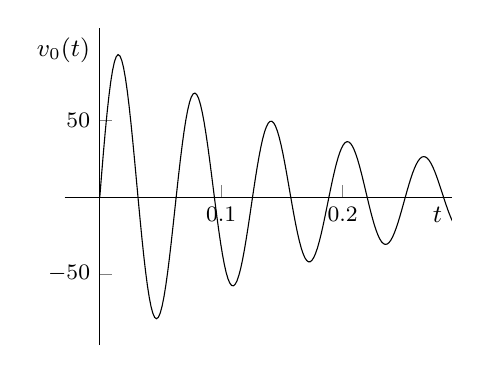
\begin{tikzpicture}
\begin{axis}[small,axis lines*=middle,xtick={0.1,0.2,0.3},xticklabels={$0.1$,$0.2$,$0.3$},xlabel={$t$},ylabel={$v_0(t)$},xlabel style={at={(current axis.right of origin)},anchor=north east},ylabel style={rotate=-90},ylabel style={at={(current axis.above origin)},anchor=north east},xmax=0.29,ytick={-50,50},yticklabels={$-50$,$50$}]
\addplot[domain=0:0.3,samples=200]{100.13*e^(-5*x)*sin(180/pi*99.87*x)};
\end{axis}
\end{tikzpicture}
\end{subfigure}%
\caption{سلسلہ وار دور (مثال \حوالہ{مثال_سلسلہ_وار_دور_اکائی_ضرب})۔}
\label{شکل_مثال_سلسلہ_وار_دور_اکائی_ضرب}
\end{figure}

حل:مسئلے کی تفرقی مساوات لکھتے ہیں
\begin{align*}
Ri(t)+L\frac{\dif i(t)}{\dif t}+\frac{1}{C}\int_{0}^{t} i(t)\dif t=Lq''+Rq'+\frac{q}{C}=\delta(t)
\end{align*}
جس کی ضمنی مساوات درج ذیل ہے جہاں برقی پرزوں کی قیمتیں بھی پر کی گئی ہیں۔
\begin{align*}
(s^2+10s+10000)Q=1
\end{align*}
ضمنی مساوات کا حل
\begin{align*}
Q=\frac{1}{(s+5)^2+9975}\approx \frac{1}{(s+5)^2+99.87^2}
\end{align*}
ہے جس کے الٹ لاپلاس بدل سے \عددی{q} حاصل کرتے ہوئے \عددی{v_0=\tfrac{q}{C}} دریافت کرتے ہیں۔
\begin{align*}
q(t)=\frac{e^{-5t}}{99.87}\sin 99.87 t\quad \implies \quad v_0(t)=\frac{q(t)}{C}=100.13e^{-5t}\sin 99.87t
\end{align*}
\انتہا{مثال}
%============================

\جزوحصہء{جزوی کسری پھیلاو پر مزید تبصرہ}
ہم نے دیکھا کہ عموماً ضمنی مساوات کی صورت \عددی{Y(s)=\tfrac{F(s)}{G(s)}} ہوتی ہے جہاں \عددی{F(s)} اور \عددی{G(s)} کثیر رکنی ہوتے ہیں۔الٹ لاپلاس بدل لیتے ہوئے حل \عددی{y(t)=\Laplace^{-1}[Y(s)]} حاصل کیا جاتا ہے۔الٹ لاپلاس بدل لینے سے پہلے کسر کو جزوی کسری پھیلاو کی مدد سے ایسی ٹکڑوں میں تقسیم کیا جاتا ہے کہ ہر ٹکڑے کا الٹ لاپلاس بدل با آسانی حاصل کرنا ممکن ہو۔

\عددی{G(s)} میں غیر دہراتا جزو \عددی{s-a} سے  جزوی کسری پھیلاو کے ذریعہ \عددی{\tfrac{A}{s-a}} رکن حاصل ہو گا جس کا الٹ لاپلاس بدل \عددی{Ae^{at}} ہے۔اسی طرح بلند درجی اجزاء \عددی{(s-a)^2} اور \عددی{(s-a)^3} درج ذیل ارکان دیتے ہیں
\begin{align*}
\frac{A_1}{(s-a)}+\frac{A_2}{(s-a)^2} \quad \text{اور} \quad \frac{A_1}{s-1}+\frac{A_2}{(s-a)^2}+\frac{A_3}{(s-a)^3}
\end{align*} 
جن کے الٹ لاپلاس بدل \عددی{(A_1+A_2t)e^{at}} اور \عددی{(A_1+A_2t+\tfrac{1}{2}A_3t^2)e^{at}} ہیں۔

\عددی{G(s)} میں غیر دہراتے مخلوط جوڑی \عددی{(s-a)(s-\bar{a})} جہاں \عددی{a=\alpha+i\beta} اور \عددی{\bar{a}=\alpha-i\beta} ہیں سے درج ذیل جزوی کسری رکن حاصل ہوتا ہے
\begin{align*}
\frac{As+B}{(s-\alpha)^2+\beta^2}
\end{align*}
جبکہ دہراتے مخلوط جوڑی مثلاً \عددی{[(s-a)(s-\bar{a})]^2} سے درج ذیل ارکان ملتے ہیں۔
\begin{align*}
\frac{As+B}{(s-\alpha)^2+\beta^2}+\frac{Cs+D}{[(s-\alpha)^2+\beta^2]^2}
\end{align*}
%============================

\ابتدا{مثال}
جزوی کسری پھیلاو استعمال کرتے ہوئے \عددی{\tfrac{3s-2}{s^2-s}} کا الٹ لاپلاس بدل حاصل کریں۔

حل:نسب نما میں \عددی{s} اور \عددی{s-1} غیر دہراتے جزو ہیں۔یوں دیے گئے تفاعل کو \عددی{\tfrac{A}{s}} اور \عددی{\tfrac{B}{s-1}} کا مجموعہ لکھا جا سکتا ہے
\begin{align*}
\frac{3s-2}{s(s-1)}=\frac{A}{s}+\frac{B}{s-1}
\end{align*}
جس میں \عددی{A} اور \عددی{B} معلوم کرنا باقی ہے۔دونوں اطراف کو \عددی{s(s-1)} سے ضرب دیتے ہوئے
\begin{align*}
3s-2=A(s-1)+Bs
\end{align*}
ملتا ہے۔اس مساوات میں \عددی{s=0} پر کرتے ہوئے \عددی{A} حاصل ہو گا جبکہ \عددی{s=1} پر کرتے ہوئے \عددی{B} حاصل ہو گا۔یوں
\begin{align*}
3(0)-2=A(0-1)+B(0)\quad \implies \quad A=2
\end{align*} 
اور
\begin{align*}
3(1)-2=A(1-1)+B(1)\quad \implies \quad B=1
\end{align*}
ملتے ہیں لہٰذا دیے گئے تفاعل کو
\begin{align*}
\frac{3s-2}{s(s-1)}=\frac{2}{s}+\frac{1}{s-1}
\end{align*}
لکھا جا سکتا ہے جس کا الٹ لاپلاس بدل درج ذیل ہے۔
\begin{align*}
\Laplace^{-1}\left(\frac{2}{s}\right)+\Laplace^{-1}\left(\frac{1}{s-1}\right)=2+e^t
\end{align*}
\انتہا{مثال}
%====================================
\ابتدا{مثال}
جزوی کسری پھیلاو استعمال کرتے ہوئے \عددی{F(s)=\tfrac{s^2-4s}{(s+2)^3}} کا الٹ لاپلاس بدل حاصل کریں۔

حل:یہاں \عددی{s+2} دہراتا جزو ہے لہٰذا درج ذیل لکھا جا سکتا ہے جس میں \عددی{A}، \عددی{B} اور \عددی{C} معلوم کرنا باقی ہے۔
\begin{align*}
\frac{s^2-4s}{(s+2)^3}=\frac{A}{s+2}+\frac{B}{(s+2)^2}+\frac{C}{(s+2)^3}
\end{align*}
دونوں اطراف کو \عددی{(s+2)^3} سے ضرب دیتے ہیں۔
\begin{align*}
s^2-4s=A(s+2)^2+B(s+2)+C
\end{align*}
\عددی{s=-2} پر کرتے ہوئے \عددی{C=12} ملتا ہے۔مساوات کا ایک درجی تفرق لے کر \عددی{s=-2} پر کرنے سے \عددی{B} حاصل ہو گا جبکہ دو درجی تفرق لے کر \عددی{s=-2} پر کرنے سے \عددی{A} حاصل ہو گا۔ یوں
\begin{align*}
2s-4&=2A(s+2)+B \implies  2(-2)-4=2A(-2+2)+B \implies  B=-8\\
2&=2A\implies  A=1
\end{align*}
ملتے ہیں۔یوں دیے گئے تفاعل کا جزوی کسری پھیلاو  اور اس کا الٹ لاپلاس بدل درج ذیل ہیں۔
\begin{align*}
F(s)&=\frac{s^2-4s}{(s+2)^3}=\frac{1}{s+2}-\frac{8}{(s+2)^2}+\frac{12}{(s+2)^3}\\
\Laplace^{-1}(F)&=e^{-2t}(1-8t+6t^2)
\end{align*}
\انتہا{مثال}
%=======================================
\ابتدا{مثال}\شناخت{مثال_لاپلاس_بدل_نیم_موج}\quad غیر دہراتے مخلوط جزو۔قصری جبری ارتعاش\\
درج ذیل اسپرنگ اور کمیت کا ابتدائی قیمت مسئلہ حل کریں۔جبری قوت \عددی{0<t<\pi} دورانیے کے لئے عمل پیرا ہے۔
\begin{align*}
y''+2y'+10y=r(t), \,\,y(0)=1, \, y'(0)=-6,\quad r(t)=
\begin{cases}
85\sin t & 0<t<\pi\\
0&t>\pi
\end{cases}
\end{align*}
حل:مسئلے کو اکائی سیڑھی تفاعل کی مدد سے لکھتے ہیں
\begin{align*}
y''+2y'+10y&=85 \sin t\, [u(t)-u(t-\pi)] \\
&=85 \sin t \,u(t)+85\sin(t-\pi)\, u(t-\pi)
\end{align*}
جہاں دائیں جزو میں \عددی{\sin t=-\sin(t-\pi)} استعمال کرتے ہوئے اس کو \عددی{f(t-a)u(t-a)} صورت میں لکھا گیا ہے۔منتقلی کا دوسرا مسئلہ استعمال کرتے ہوئے اس کا ضمنی مساوات لکھتے ہیں۔
\begin{align*}
[s^2Y-s(1)+6]+2[sY-1]+10Y=85\frac{1}{s^2+1}(1+e^{-\pi s})
\end{align*}
جسے  \عددی{Y} کے لئے حل کرتے ہیں۔
\begin{align}\label{مساوات_مثال_لاپلاس_نصف_لہر_الف}
Y=\frac{85}{(s^2+1)(s^2+2s+10)}+\frac{85}{(s^2+1)(s^2+2s+10)}e^{-\pi s}+\frac{s-4}{s^2+2s+10}
\end{align}
منتقلی کے پہلے مسئلے سے مساوات \حوالہ{مساوات_مثال_لاپلاس_نصف_لہر_الف} کے آخری جزو کا الٹ لاپلاس بدل لکھتے ہیں۔
\begin{align}\label{مساوات_مثال_لاپلاس_نصف_لہر_ب}
\Laplace^{-1}\left[\frac{s-4}{s^2+2s+10}\right]=\Laplace^{-1}\left[\frac{(s+1)-5}{(s+1)^2+3^2}\right]=e^{-t}(\cos 3t-\frac{5}{3}\sin 3t)
\end{align}
مساوات \حوالہ{مساوات_مثال_لاپلاس_نصف_لہر_الف} کے پہلے جزو میں غیر دہراتے مخلوط جذر پائے جاتے ہیں لہٰذا اس کا جزوی کسری پھیلاو درج ذیل ہو گا جہاں \عددی{A}، \عددی{B}، \عددی{C} اور \عددی{D} معلوم کرنا باقی ہے۔
\begin{align*}
\frac{85}{(s^2+1)(s^2+2s+10)}=\frac{As+B}{s^2+1}+\frac{Cs+D}{s^2+2s+10}
\end{align*}
دونوں اطراف کو \عددی{s^2+1)(s^2+2s+10)} سے ضرب دیتے ہیں۔
\begin{align*}
85=(As+B)(s^2+2s+10)+(Cs+D)(s^2+1)
\end{align*}
ہر \عددی{s} کے دونوں اطراف کے عددی سروں کو آپس میں برابر لکھتے
\begin{align*}
& s^3:\quad A+C=0, & s^2:\quad 2A+B+D=0\\
& s^1:\quad 10A+2B+C=0, & s^0:\quad 10B+D=85
\end{align*} 
ہوئے چار عدد ہمزاد مساوات حاصل ہوتے ہیں جن کا حل \عددی{A=-2}، \عددی{B=9}، \عددی{C=2} اور \عددی{D=-5} ہے۔یوں مساوات \حوالہ{مساوات_مثال_لاپلاس_نصف_لہر_الف} کے پہلے جزو کا جزوی کسری پھیلاو درج ذیل ہو گا
\begin{align*}
\frac{-2s+9}{s^2+1}+\frac{2(s+1)-7}{(s+1)^2+9}
\end{align*}
جس کا الٹ لاپلاس بدل درج ذیل ہے۔
\begin{align}\label{مساوات_مثال_لاپلاس_نصف_لہر_پ}
-2\cos t+9\sin t+e^{-t}(2\cos 3t-\frac{7}{3}\sin 3t)
\end{align}
مساوات \حوالہ{مساوات_مثال_لاپلاس_نصف_لہر_ب} اور مساوات \حوالہ{مساوات_مثال_لاپلاس_نصف_لہر_پ} کا مجموعہ \عددی{0<t<\pi} دورانیے کا حل ہے۔
\begin{align}\label{مساوات_مثال_لاپلاس_نصف_لہر_ت}
y(t)=e^{-t}(3\cos 3t-4\sin 3t)-2\cos t+9\sin t\quad 0<t<\pi
\end{align}
مساوات \حوالہ{مساوات_مثال_لاپلاس_نصف_لہر_الف} کے دوسرے جزو میں  \عددی{e^{-\pi s}} پایا جاتا ہے لہٰذا مساوات \حوالہ{مساوات_مثال_لاپلاس_نصف_لہر_پ} اور منتقلی کے دوسرے مسئلے سے \عددی{t>\pi} کے لئے  اس کا الٹ لاپلاس بدل درج ذیل ہو گا
\begin{align*}
-2\cos (t-\pi)+9\sin (t-\pi)+e^{-(t-\pi)}[2\cos 3(t-\pi)-\frac{7}{3}\sin 3(t-\pi)]
\end{align*}
جس میں \عددیء{\cos(t-\pi)=-\cos t} اور   \عددیء{\cos(3t-3\pi)=-\cos 3t}، \نقطے استعمال کرتے ہوئے
\begin{align*}
2\cos t-9\sin t+e^{-(t-\pi)}[-2\cos 3t+\frac{7}{3}\sin 3t]
\end{align*}
ملتا ہے۔اس کو مساوات \حوالہ{مساوات_مثال_لاپلاس_نصف_لہر_ت}  کے ساتھ جمع کرنے سے \عددی{t>\pi} پر مسئلے کا حل ملتا ہے۔
\begin{multline}
y(t)=e^{-t}(3\cos 3t-4\sin 3t)+e^{-(t-\pi)}(-2\cos 3t+\frac{7}{3}\sin 3t) \quad t>\pi
\end{multline} 
شکل \حوالہ{شکل_مثال_لاپلاس_بدل_نیم_موج} میں مسئلے کا حل دکھایا گیا ہے۔
\begin{figure}
\centering
\begin{tikzpicture}
\begin{axis}[small,axis lines*=middle,xtick={3.1412,6.2824},xticklabels={$\pi$,$2\pi$},xlabel={$t$},xlabel style={at={(current axis.right of origin)},anchor=north east}]
\addplot[domain=0:pi,samples=100]{e^(-x)*(3*cos(180/pi*3*x)-4*sin(180/pi*3*x))-2*cos(180/pi*x)+9*sin(180/pi*x)};
\addplot[domain=pi:9,samples=100]{e^(-x)*(3*cos(180/pi*3*x)-4*sin(180/pi*3*x))+e^(-(x-pi))*(-2*cos(180/pi*3*x)+7/3*sin(180/pi*3*x))};
\end{axis}
\end{tikzpicture}
\caption{اسپرنگ اور کمیت کا جبری ارتعاش (مثال \حوالہ{مثال_لاپلاس_بدل_نیم_موج})۔}
\label{شکل_مثال_لاپلاس_بدل_نیم_موج}
\end{figure}
\انتہا{مثال}
%======================================
\حصہء{سوالات}
سوال \حوالہ{سوال_لاپلاس_ابتدائی_قیمت_مسئلہ_الف} تا سوال \حوالہ{سوال_لاپلاس_ابتدائی_قیمت_مسئلہ_الف} ابتدائی قیمت مسئلے ہیں۔ انہیں حل کریں۔

%==================
\ابتدا{سوال}\شناخت{سوال_لاپلاس_ابتدائی_قیمت_مسئلہ_الف}\quad
$y''+y=\delta(t-\pi),\quad y(0)=4, \, y'(0)=0$\\
جواب:\عددی{y=4\cos t-u(t-\pi)\, \sin t}؛ اکائی ضرب عین \عددی{t=\pi} پر عمل کرتی ہے۔ابتدائی معلومات صرف اس صورت ممکن ہیں کہ اکائی ضرب سے پہلے بھی نظام ارتعاش پذیر ہو۔جواب میں \عددی{4\cos t} اسی ارتعاش کو ظاہر کرتی ہے۔ 
\انتہا{سوال}
%====================
\ابتدا{سوال}\quad
$y''+y=2\delta(t-3\pi),\quad y(0)=1, \, y'(0)=0$\\
جواب:\عددی{y=\cos t-2u(t-3\pi)\sin t}
\انتہا{سوال}
%==================
\ابتدا{سوال}\quad
$y''+4y=3\delta(t-2\pi),\quad y(0)=-2, \, y'(0)=1$\\
جواب:\عددی{y=2\cos 2t+0.5\sin 2t+1.5u(t-2\pi)\sin t}
\انتہا{سوال}
%==================
\ابتدا{سوال}\quad
$y''+9y=2\delta(t-\pi)-\delta(t-2\pi),\quad y(0)=0, \, y'(0)=-1$\\
جواب:\عددی{y=-\tfrac{1}{3}\sin 3t-\tfrac{2}{3}u(t-\pi)\sin 3t-\tfrac{1}{3}u(t-2\pi)\sin 3t}
\انتہا{سوال}
%======================
\ابتدا{سوال}\quad
$y''+6y'+10y=\delta(t-1), \quad y(0)=0,\, y'(0)=2$\\
جواب:\عددی{y=2e^{-3t}\sin t+e^{-3(t-1)}u(t-1)\sin (t-1)}
\انتہا{سوال}
%========================
\ابتدا{سوال}\quad
$2y''+3y'+y=2e^{-t}+\delta(t-1), \quad y(0)=0, \, y'(0)=1$\\
جواب:\عددی{y=6e^{-\tfrac{t}{2}}-e^{-t}(6+2t)+4u(t-1)[e^{-\tfrac{1}{2}(t-1)}-e^{-(t-1)}]}
\انتہا{سوال}
%=======================
\ابتدا{سوال}\quad
$y''+3y'+3y=5\sin t+20\delta(t-1),\quad y(0)=1,\, y'(0)=1$\\
جواب:\عددی{y=\sin t-3\cos t+8e^{-t}-4e^{-2t}+[e^{-(t-1)}-e^{-2(t-1)}]u(t-1)}
\انتہا{سوال}
%=======================
\ابتدا{سوال}\quad
$y''+4y'+5y=[u(t)-u(t-2)]e^t-6\delta(t-3), y(0)=0, y'(0)=1$\\
دائیں ہاتھ پہلا جزو درج ذیل لکھتے ہوئے آگے چلیں۔
\begin{align*}
[u(t)-u(t-2)]e^t=u(t)e^t-e^2u(t-2)e^{(t-2)}
\end{align*}
یوں جواب درج ذیل ملتا ہے۔
\begin{multline*}
y=\frac{1}{5}e^{-2t}(3\sin t-\cos t)+\frac{1}{5}+\frac{e^2e^{-2(t-2)}}{5}[2\sin(t-2)+\cos(t-2)]u(t-2)\\
-\frac{e^2}{5}u(t-2)-6e^{-2(t-3)}\sin(t-3)u(t-3)
\end{multline*}
\انتہا{سوال}
%=====================
